\documentclass[aspectratio=169,12pt,handout]{beamer}
\usepackage{pgfpages}
\pgfpagesuselayout{resize to}[letterpaper,landscape,border shrink=5mm]
\usetheme{Madrid}
\usecolortheme{default}
\usepackage{graphicx}
\usepackage{booktabs}
\usepackage{amsmath}

% Clean colors
\definecolor{binggreen}{RGB}{0,100,0}
\setbeamercolor{structure}{fg=binggreen}
\setbeamercolor{title}{fg=white,bg=binggreen}
\setbeamercolor{frametitle}{fg=white,bg=binggreen}

\setbeamertemplate{navigation symbols}{}
\setbeamertemplate{footline}[frame number]

\hypersetup{pdfpagelayout=SinglePage}

\title{Gene Expression Pattern Matching}
\subtitle{Evaluating Similarity Metrics for NMF Constraint Patterns}
\author{}
\institute{Binghamton University}
\date{April 2026}

\begin{document}

% ------------------------------------------------------------------
\begin{frame}
\titlepage
\end{frame}

% ------------------------------------------------------------------
\begin{frame}{Motivation}
\begin{itemize}
  \item \textbf{Goal:} Identify genes whose expression over time matches
        biologically observed constraint patterns
  \item \textbf{Data:} $\sim$17,856 genes across 4 timepoints (0, 3, 6, 9)
        in 4 clusters, raw and log-transformed
  \item \textbf{Problem with NMF:} All factors are non-negative, so NMF
        ranks genes by coefficient magnitude, not shape match.
        Up-regulation and down-regulation are conflated.
  \item \textbf{Our approach:} Compare 6 similarity metrics that directly
        measure gene--pattern shape similarity
\end{itemize}
\end{frame}

% ------------------------------------------------------------------
\begin{frame}{Constraint Patterns}
\begin{center}
\begin{tabular}{lccccl}
\toprule
\textbf{Cluster} & \textbf{t=0} & \textbf{t=3} & \textbf{t=6} & \textbf{t=9} & \textbf{Shape} \\
\midrule
One   & 1.45  & 12.0  & 5.21  & 6.51  & Spike at t=3 \\
Two   & 0.371 & 0.803 & 1.22  & 1.78  & Steady increase \\
Three & 0.041 & 0.0   & 0.037 & 0.035 & Near-flat, dip at t=3 \\
Four  & 0.009 & 0.638 & 0.018 & 0.024 & 70$\times$ spike at t=3 \\
\bottomrule
\end{tabular}
\end{center}

\vspace{0.5em}
\small
All data min-max normalized to $(0, 1]$ before comparison.
Both raw and log-transformed (LT) versions analyzed.
\end{frame}

% ------------------------------------------------------------------
\begin{frame}{The 6 Metrics at a Glance}
\begin{center}
\small
\begin{tabular}{llll}
\toprule
\textbf{Metric} & \textbf{Measures} & \textbf{Ranking} & \textbf{Key property} \\
\midrule
Pearson  & Shape (mean-centered) & Higher = better & Scale \& shift invariant \\
Cosine   & Vector angle (raw)    & Higher = better & No mean-centering \\
DTW      & Time-aligned distance & Lower = better  & Allows temporal warping \\
Fr\'{e}chet & Max curve deviation   & Lower = better  & Worst-point sensitive \\
MSE      & Avg squared error     & Lower = better  & Simplest distance \\
sMAPE    & Symmetric \% error    & Lower = better  & Relative scale \\
\bottomrule
\end{tabular}
\end{center}
\end{frame}

% ------------------------------------------------------------------
\begin{frame}{Pearson Correlation --- Primary Metric}
$$r = \frac{\sum(p_i - \bar{p})(g_i - \bar{g})}
           {\sqrt{\sum(p_i - \bar{p})^2 \cdot \sum(g_i - \bar{g})^2}}$$

\begin{itemize}
  \item Mean-centers both vectors $\Rightarrow$ measures \textbf{shape only}
  \item Scale and shift invariant: $[1, 12, 5, 7]$ and $[100, 1200, 500, 700]$
        get the same score
  \item Best fit for the biological question: ``does this gene go up when the
        pattern goes up?''
  \item \textbf{Caveat:} with $n=4$, there is a $\sim$20\% chance of $|r|>0.8$
        under the null --- interpret rankings, not absolute values
\end{itemize}
\end{frame}

% ------------------------------------------------------------------
\begin{frame}{Why Cosine Similarity Diverges from Pearson}
$$\cos(\theta) = \frac{\sum p_i g_i}{\sqrt{\sum p_i^2}\sqrt{\sum g_i^2}}$$

\begin{itemize}
  \item Same formula as Pearson but \textbf{without mean-centering}
  \item A flat gene $[1, 1, 1, 1]$ gets high cosine with almost any positive pattern
  \item Finds housekeeping genes (high, stable expression) instead of shape-matching genes
  \item Behavior is \textbf{context-dependent}: perfect overlap with Pearson on clusterThree (20/20),
        but only 2/20 on clusterOne
\end{itemize}
\end{frame}

% ------------------------------------------------------------------
\begin{frame}{DTW, Fr\'{e}chet, MSE --- Distance Metrics}
\begin{columns}[T]
\begin{column}{0.33\textwidth}
\textbf{DTW}\\[0.5em]
Finds optimal temporal alignment.
At 4 timepoints, warping is minimal
$\Rightarrow$ largely redundant with pointwise methods.
\end{column}
\begin{column}{0.33\textwidth}
\textbf{Fr\'{e}chet}\\[0.5em]
Worst-case pointwise deviation
(``dog-walking distance'').
At $n=4$, behaves very similarly to MSE.
\end{column}
\begin{column}{0.33\textwidth}
\textbf{MSE}\\[0.5em]
Average squared error.
After normalization, approximately
inversely related to Pearson:\\
$\text{MSE} \approx 2\sigma^2(1-r)$.
\end{column}
\end{columns}

\vspace{1em}
\textbf{Key insight:} Fr\'{e}chet and MSE are near-redundant (19--20/20 overlap).
Both confirm Pearson's findings from a distance perspective.
\end{frame}

% ------------------------------------------------------------------
\begin{frame}{sMAPE --- Failure Mode at Zero Values}
$$\text{sMAPE} = \frac{1}{n}\sum \frac{2|p_i - g_i|}{|p_i| + |g_i|}$$

\begin{itemize}
  \item Measures \textbf{relative} (percentage) error per timepoint
  \item When $p_i = 0$: $\text{sMAPE}_i = 2|g_i|/|g_i| = 2.0$ regardless of $g_i$
  \item clusterThree has a zero at $t=3$ $\Rightarrow$ sMAPE cannot discriminate
        at the most informative timepoint
  \item Result: \textbf{0/20 overlap} with every other method on clusterThree
\end{itemize}
\end{frame}

% ------------------------------------------------------------------
\begin{frame}{Results: clusterTwo LT --- Best Agreement}
\begin{columns}[T]
\begin{column}{0.45\textwidth}
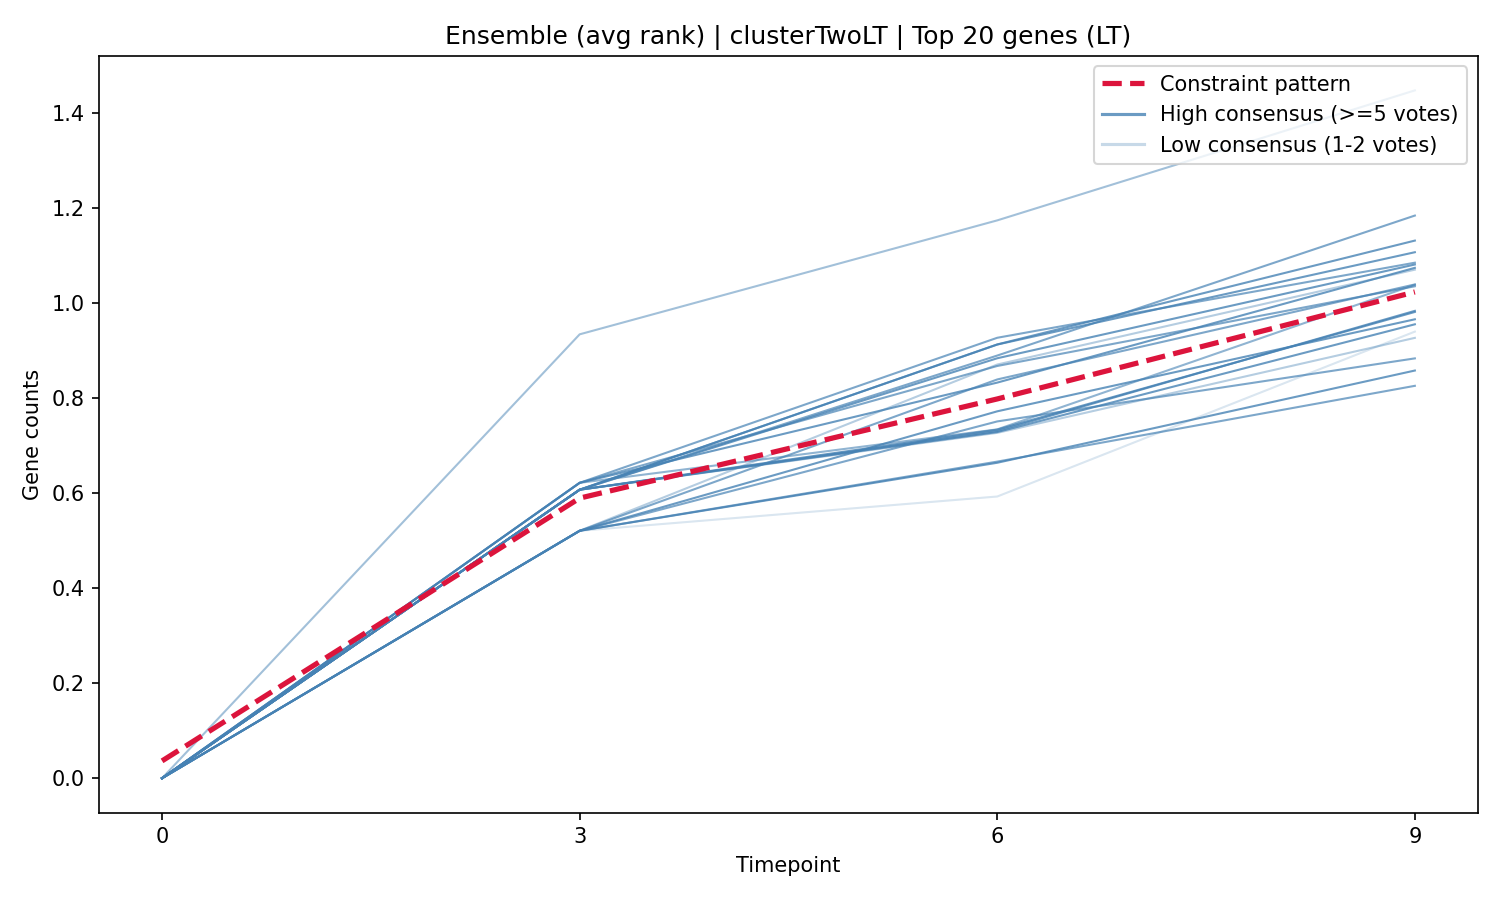
\includegraphics[width=\textwidth]{plots/Ensemble_LT_clusterTwoLT_constraint.png}
\end{column}
\begin{column}{0.52\textwidth}
\small
\textbf{9 of top 11 genes} achieve unanimous 6/6 votes:\\[0.3em]
RAB14, SYNGR1, ARHGAP25,\\
HNRNPH3, BSG, CAPN2,\\
NOL7, ZC3H15, PRDX6\\[0.5em]
Steady-increase pattern is easiest
to match --- all methods converge.\\[0.5em]
\textbf{Highest-confidence candidates}\\for biological follow-up.
\end{column}
\end{columns}
\end{frame}

% ------------------------------------------------------------------
\begin{frame}{Results: clusterThree --- Strong Consensus (Except sMAPE)}
\begin{columns}[T]
\begin{column}{0.45\textwidth}
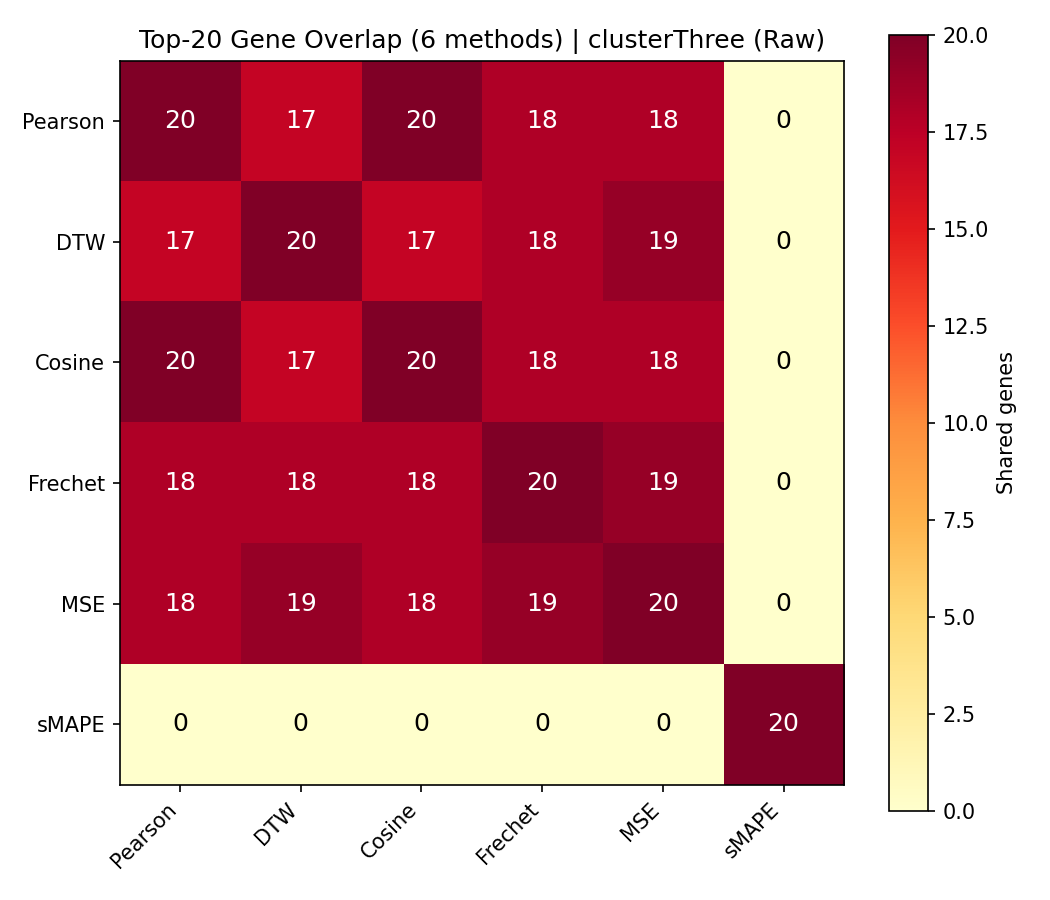
\includegraphics[width=\textwidth]{plots/overlap_6methods_clusterThree.png}
\end{column}
\begin{column}{0.52\textwidth}
\small
Pearson, DTW, Cosine, Fr\'{e}chet, MSE\\
all agree: 17--20/20 overlap.\\[0.5em]
sMAPE: 0/20 overlap with everything\\
(zero-value failure at $t=3$).\\[0.5em]
Consensus genes: TEDC1, PGAP1, TANGO6\\[0.5em]
\textbf{Validates that 5 of 6 methods\\capture the same biology.}
\end{column}
\end{columns}
\end{frame}

% ------------------------------------------------------------------
\begin{frame}{Results: clusterOne --- Pearson/MSE/Fr\'{e}chet Core}
\begin{columns}[T]
\begin{column}{0.45\textwidth}
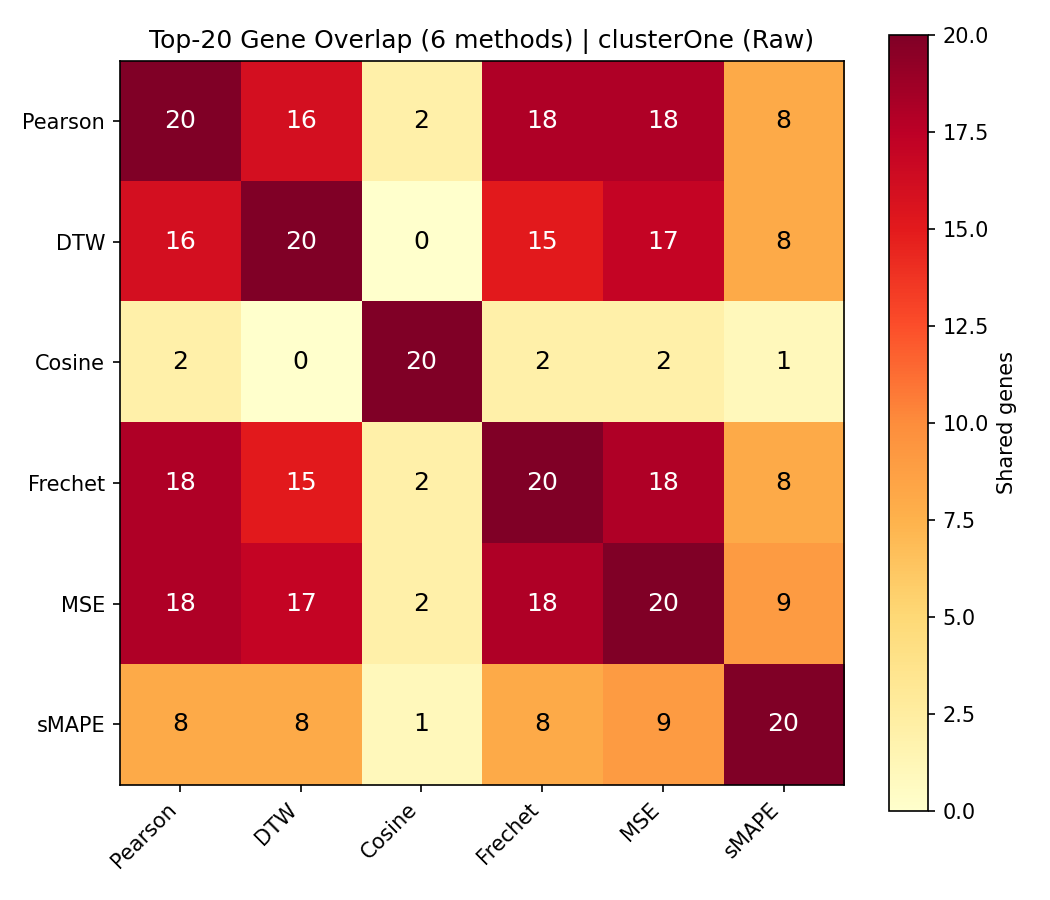
\includegraphics[width=\textwidth]{plots/overlap_6methods_clusterOne.png}
\end{column}
\begin{column}{0.52\textwidth}
\small
Pearson--MSE--Fr\'{e}chet: 18/20 overlap\\
DTW joins at 15--17/20\\
Cosine isolated: 0--2/20\\[0.5em]
Top ensemble genes (5/6 votes):\\
SSR3, REXO2, YIF1A, MAZ,\\
ACBD3, GSPT2\\[0.5em]
Cosine finds magnitude, not shape.
\end{column}
\end{columns}
\end{frame}

% ------------------------------------------------------------------
\begin{frame}{Results: clusterFour --- The Hard Case}
\begin{columns}[T]
\begin{column}{0.45\textwidth}
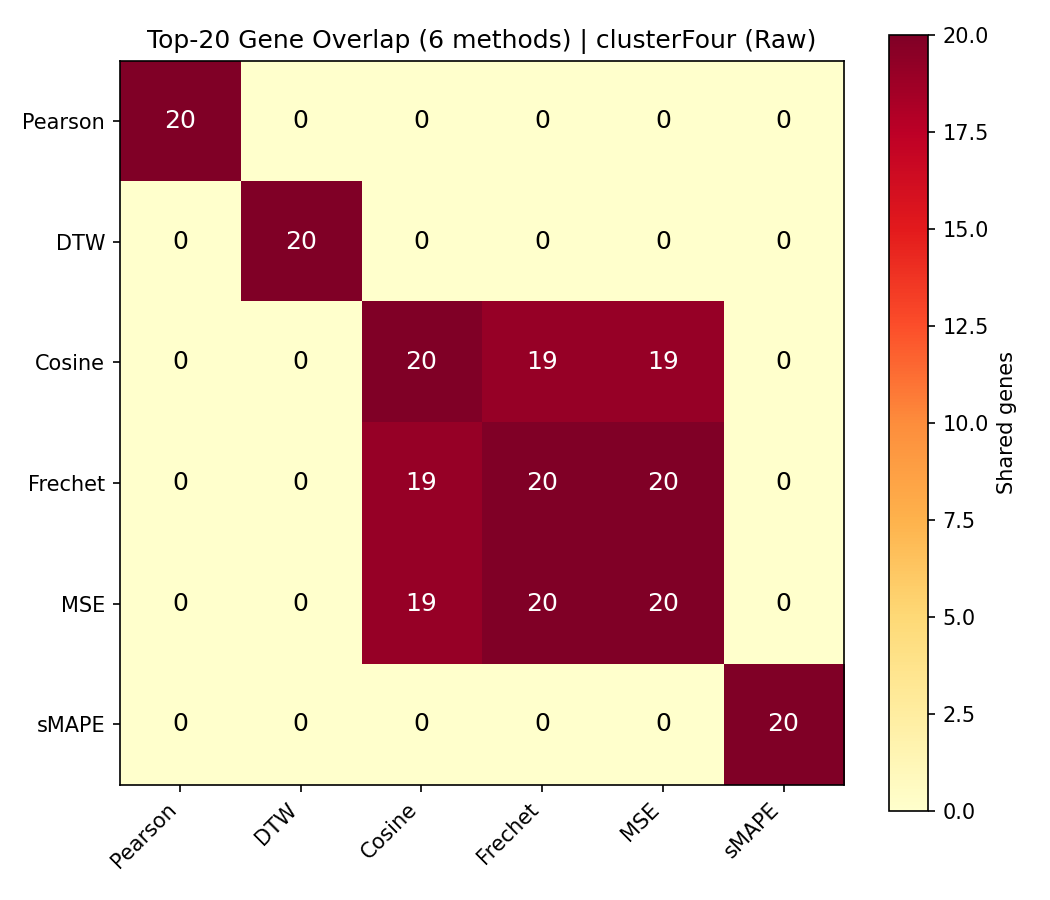
\includegraphics[width=\textwidth]{plots/overlap_6methods_clusterFour.png}
\end{column}
\begin{column}{0.52\textwidth}
\small
70$\times$ spike $\Rightarrow$ effectively a delta function.\\[0.3em]
Cosine/Fr\'{e}chet/MSE agree (19--20/20):\\
all dominated by $t=3$ magnitude.\\[0.3em]
Pearson isolated (scale-invariant,\\
finds \textit{relative} peaks).\\[0.3em]
DTW, sMAPE also isolated.\\[0.5em]
\textbf{No genuine shape consensus.}\\
Needs denser time sampling to resolve.
\end{column}
\end{columns}
\end{frame}

% ------------------------------------------------------------------
\begin{frame}{Pearson vs Cosine --- Visual Comparison (clusterOne LT)}
\begin{columns}[T]
\begin{column}{0.48\textwidth}
\centering
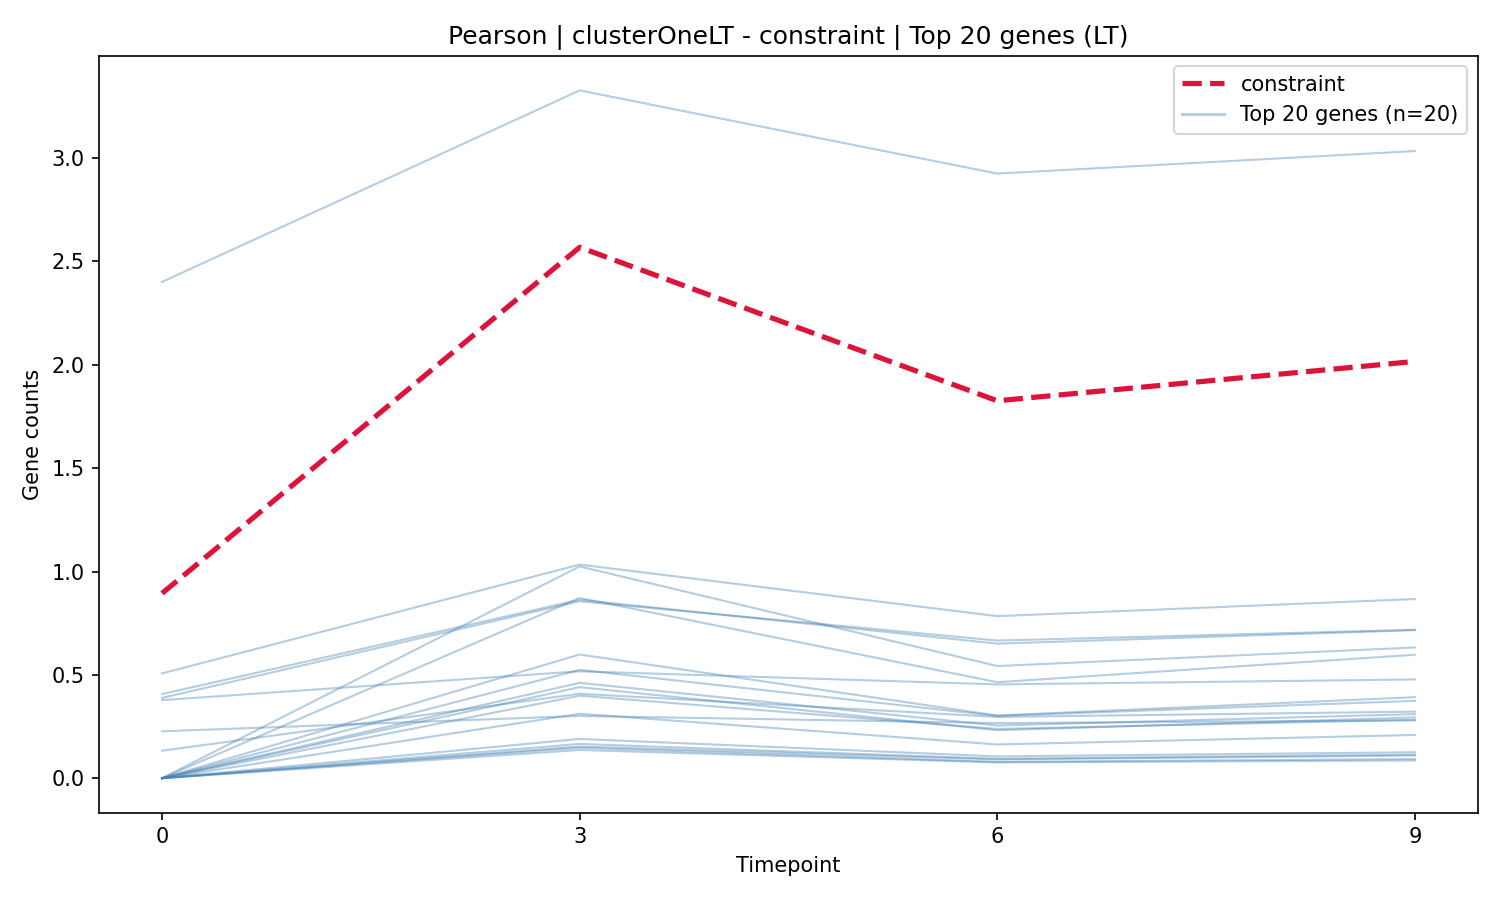
\includegraphics[width=\textwidth]{plots/Pearson_LT_clusterOneLT_constraint.png}\\
\small Pearson: shape-matching genes
\end{column}
\begin{column}{0.48\textwidth}
\centering
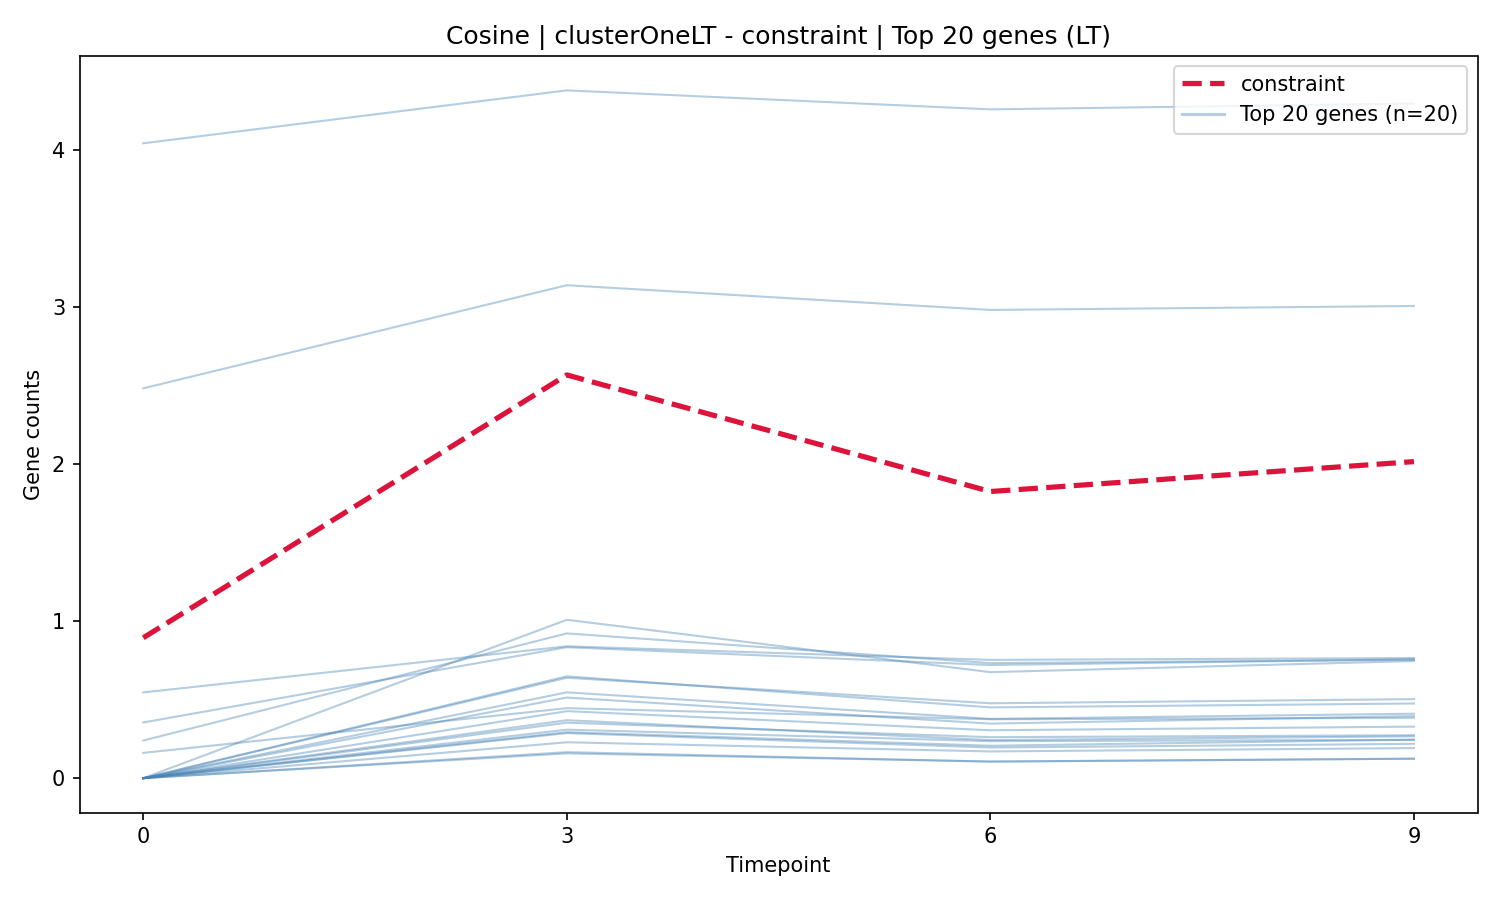
\includegraphics[width=\textwidth]{plots/Cosine_LT_clusterOneLT_constraint.png}\\
\small Cosine: magnitude-biased genes
\end{column}
\end{columns}
\end{frame}

% ------------------------------------------------------------------
\begin{frame}{Ensemble Rankings --- clusterTwo (Raw)}
\small
\begin{center}
\begin{tabular}{clcl}
\toprule
\textbf{Rank} & \textbf{Gene} & \textbf{Votes} & \textbf{Methods} \\
\midrule
1 & FAM49B  & \textbf{6/6} & All methods \\
2 & RNF213  & \textbf{6/6} & All methods \\
3 & ARGLU1  & 4/6 & Pearson, DTW, Fr\'{e}chet, MSE \\
4 & TMC8    & 5/6 & Pearson, Cosine, Fr\'{e}chet, MSE, sMAPE \\
5 & SNRNP70 & 5/6 & Pearson, Cosine, Fr\'{e}chet, MSE, sMAPE \\
\bottomrule
\end{tabular}
\end{center}

\vspace{0.5em}
FAM49B and RNF213 are unanimous across all 6 methods --- highest confidence
candidates for TCR pathway involvement.
\end{frame}

% ------------------------------------------------------------------
\begin{frame}{Recommendations}
\begin{enumerate}
  \item \textbf{Primary metric:} Pearson --- directly captures shape, invariant
        to scale and baseline
  \item \textbf{Secondary validation:} MSE --- independent distance-based
        confirmation (Fr\'{e}chet is near-redundant with MSE)
  \item \textbf{Skip for this data:} Cosine (inconsistent), sMAPE (zero-point failure)
  \item \textbf{DTW:} marginal benefit at 4 timepoints; valuable with denser sampling
  \item \textbf{Ensemble:} 3-method consensus (Pearson + DTW + MSE), $\geq$2/3 agreement
        for high-confidence gene lists
  \item \textbf{clusterFour:} needs more timepoints or peak-detection approach
\end{enumerate}
\end{frame}

% ------------------------------------------------------------------
\begin{frame}{}
\vfill
\centering
\textbf{\Huge Thank you}
\vfill
\end{frame}

% ==================================================================
% APPENDIX: All Methods — LT Clusters
% ==================================================================
\appendix
\begin{frame}{}
\centering
\vfill
{\Huge\textbf{Appendix}}\\[1em]
{\large All Methods — Log-Transformed Clusters}
\vfill
\end{frame}

% --- clusterOne LT ---
\begin{frame}{clusterOne LT — Pearson}
\centering
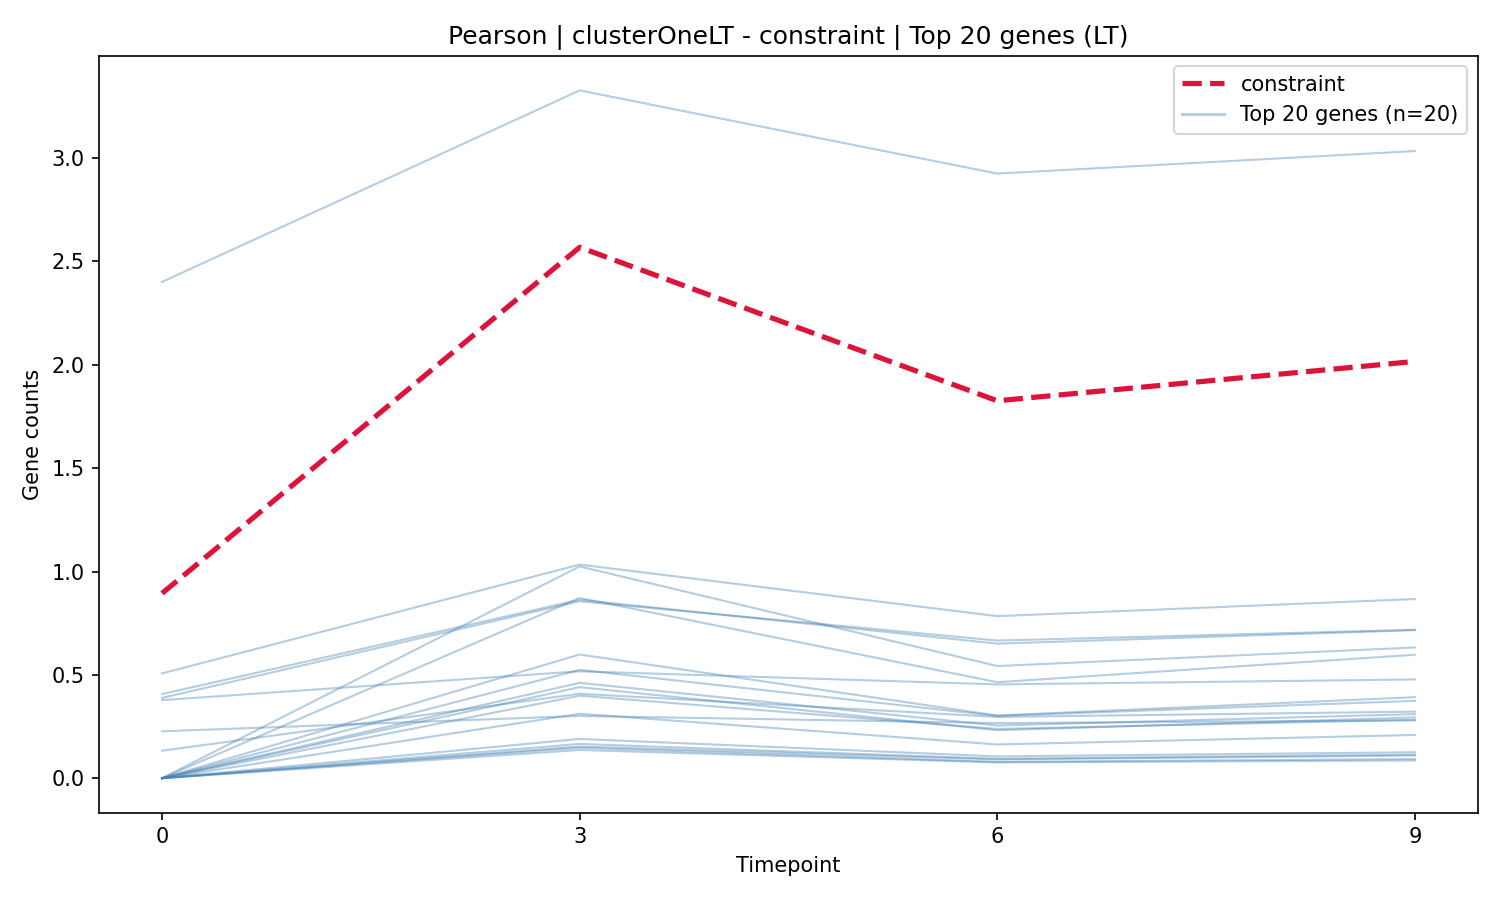
\includegraphics[height=0.85\textheight]{plots/Pearson_LT_clusterOneLT_constraint.png}
\end{frame}

\begin{frame}{clusterOne LT — DTW}
\centering
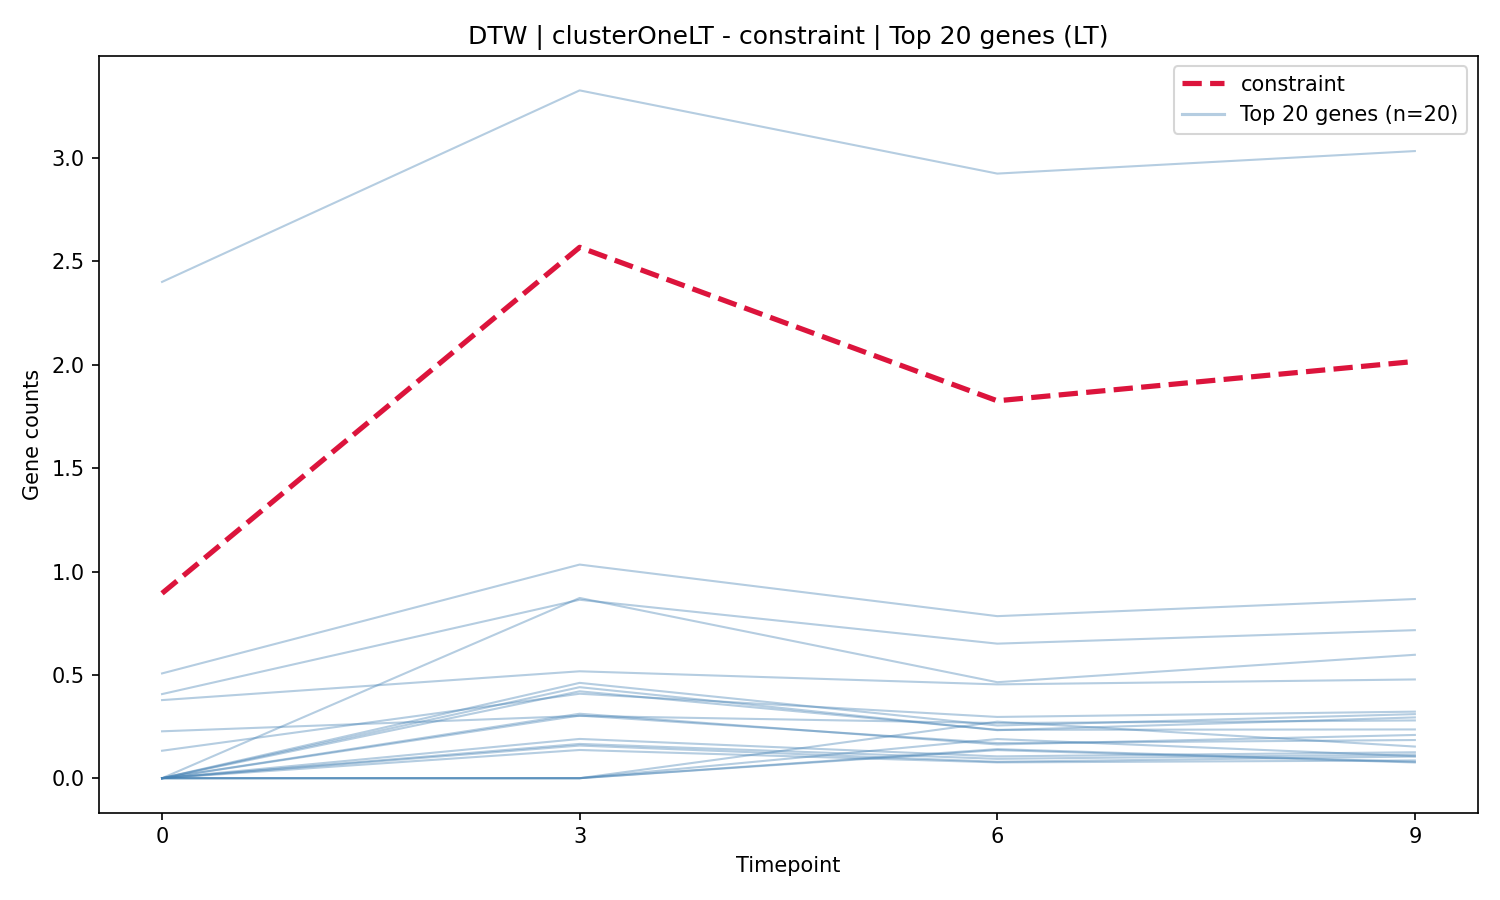
\includegraphics[height=0.85\textheight]{plots/DTW_LT_clusterOneLT_constraint.png}
\end{frame}

\begin{frame}{clusterOne LT — Cosine}
\centering
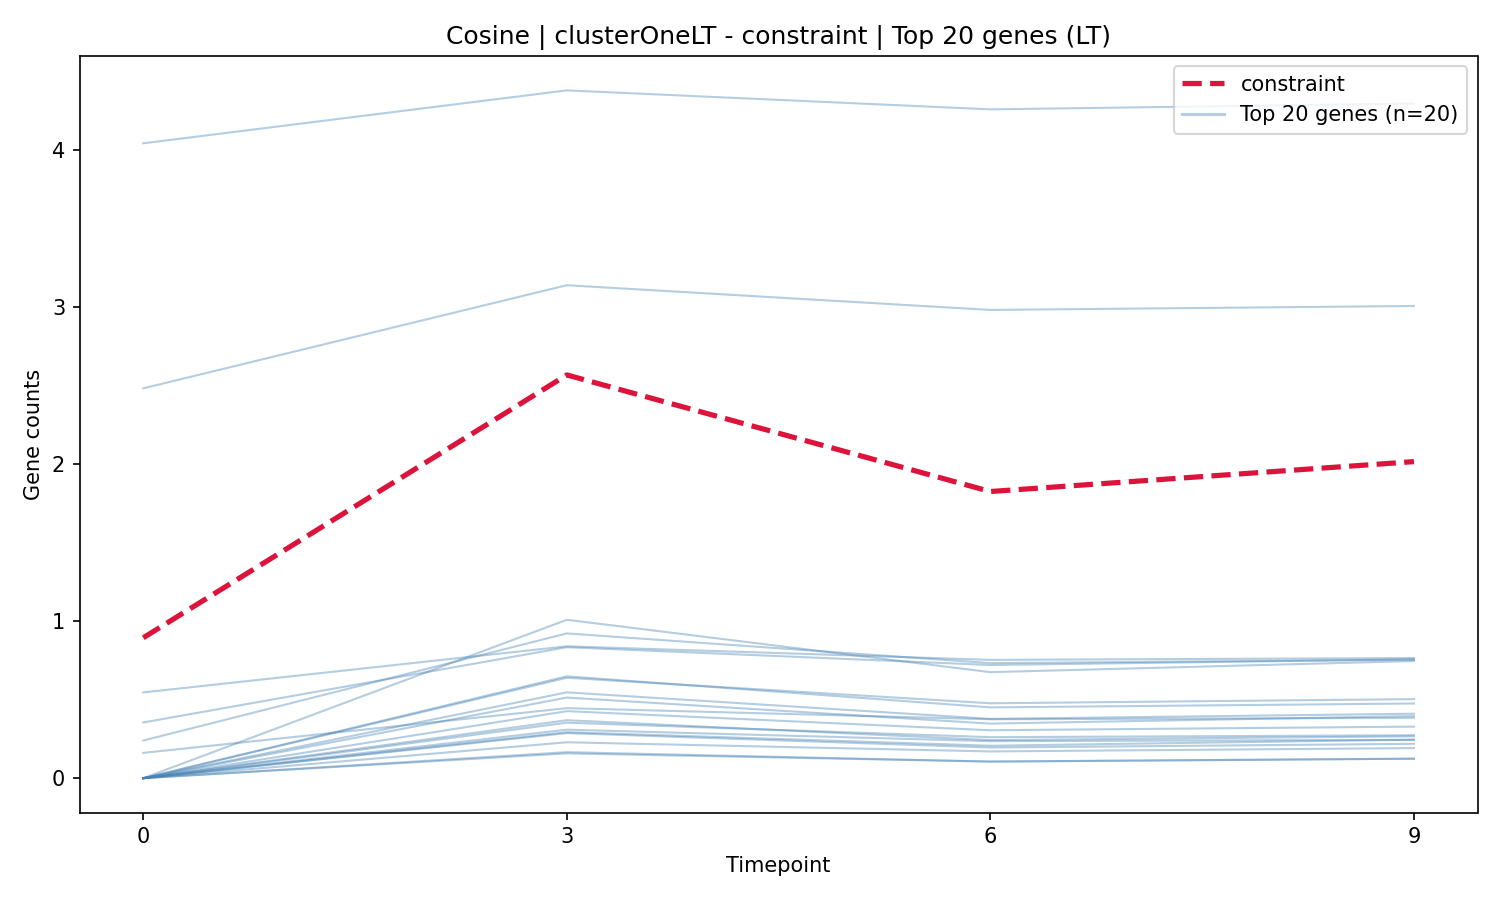
\includegraphics[height=0.85\textheight]{plots/Cosine_LT_clusterOneLT_constraint.png}
\end{frame}

\begin{frame}{clusterOne LT — Fr\'{e}chet}
\centering
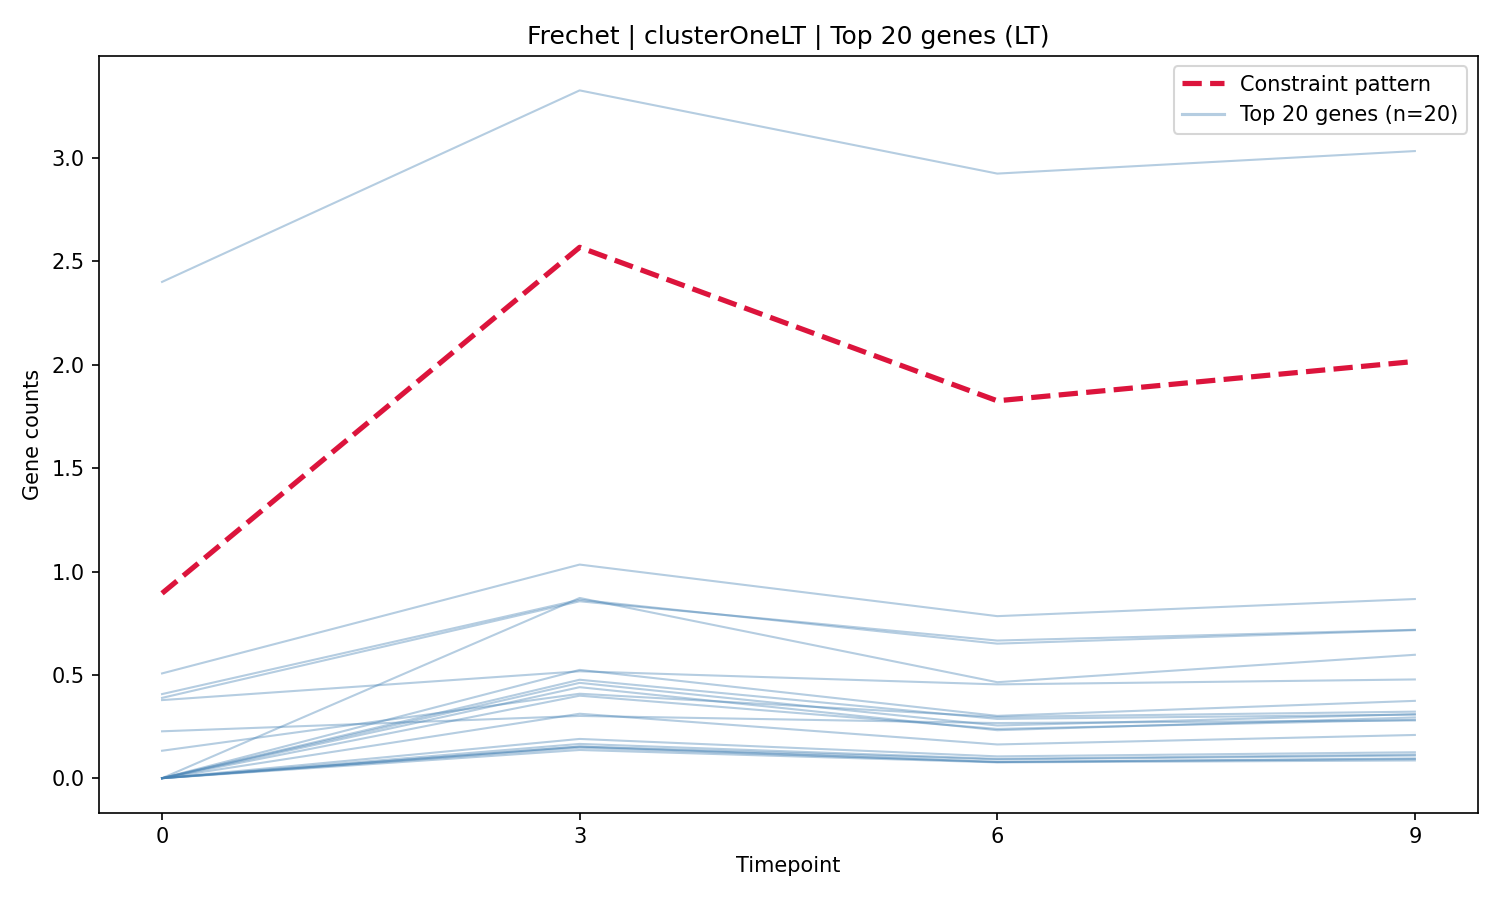
\includegraphics[height=0.85\textheight]{plots/Frechet_LT_clusterOneLT_constraint.png}
\end{frame}

\begin{frame}{clusterOne LT — MSE}
\centering
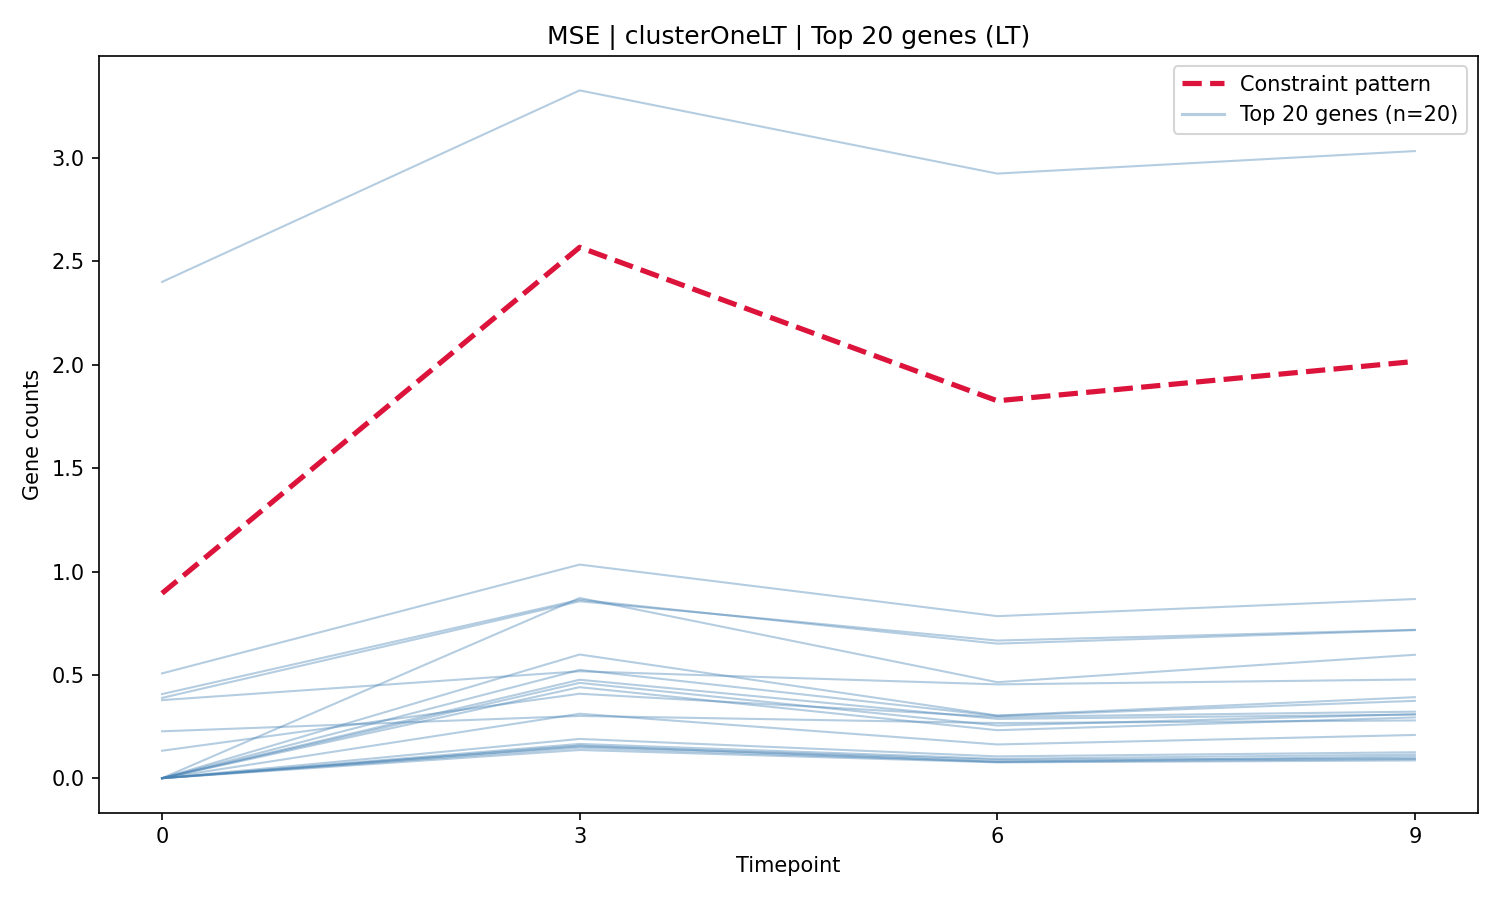
\includegraphics[height=0.85\textheight]{plots/MSE_LT_clusterOneLT_constraint.png}
\end{frame}

\begin{frame}{clusterOne LT — sMAPE}
\centering
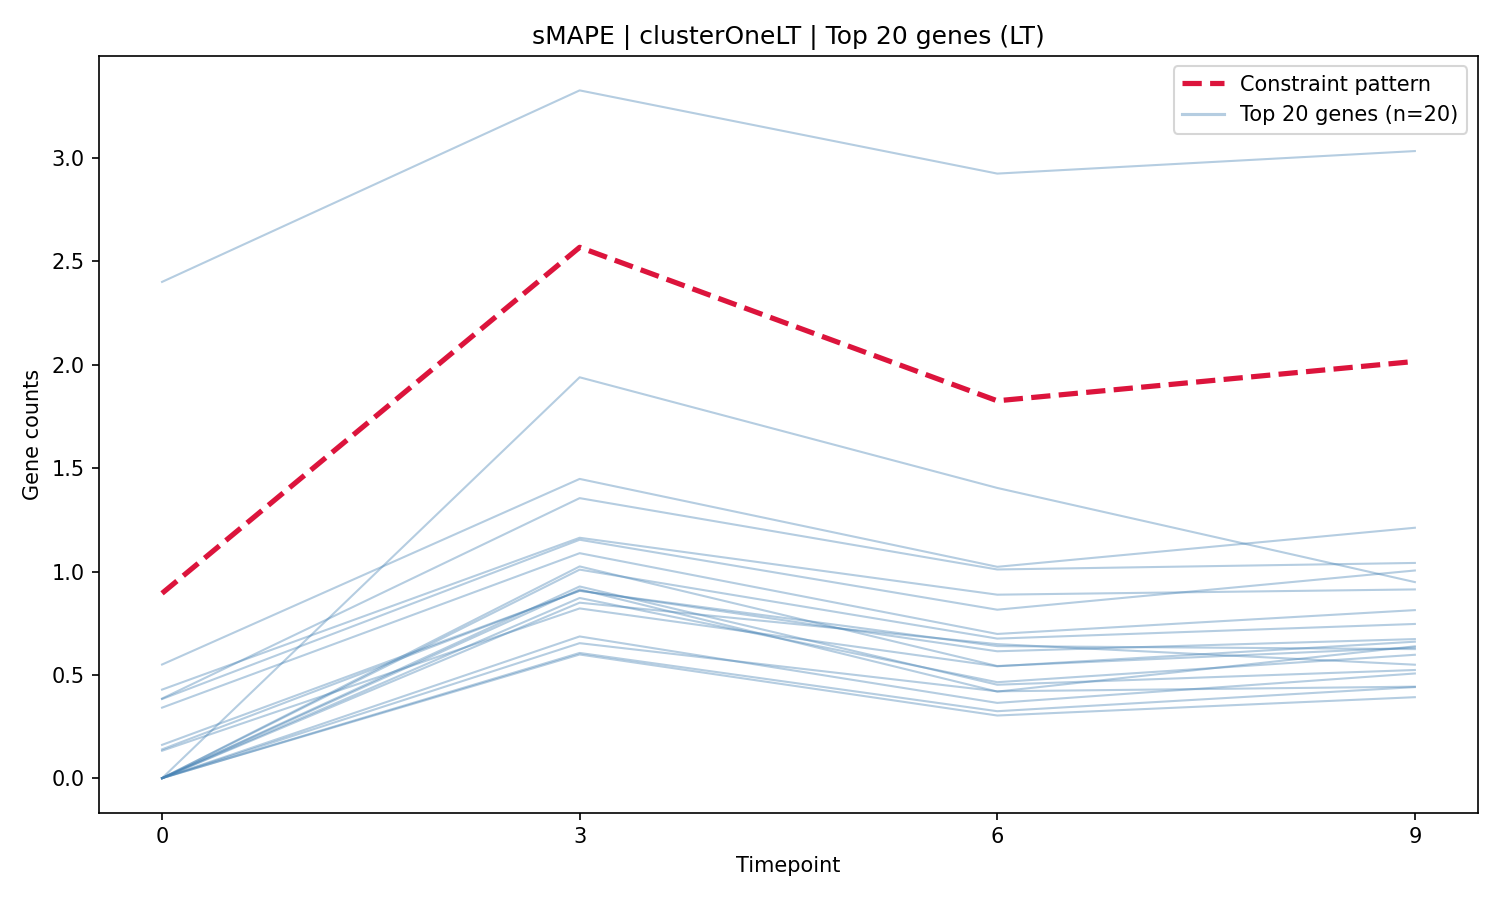
\includegraphics[height=0.85\textheight]{plots/sMAPE_LT_clusterOneLT_constraint.png}
\end{frame}

\begin{frame}{clusterOne LT — Ensemble}
\centering
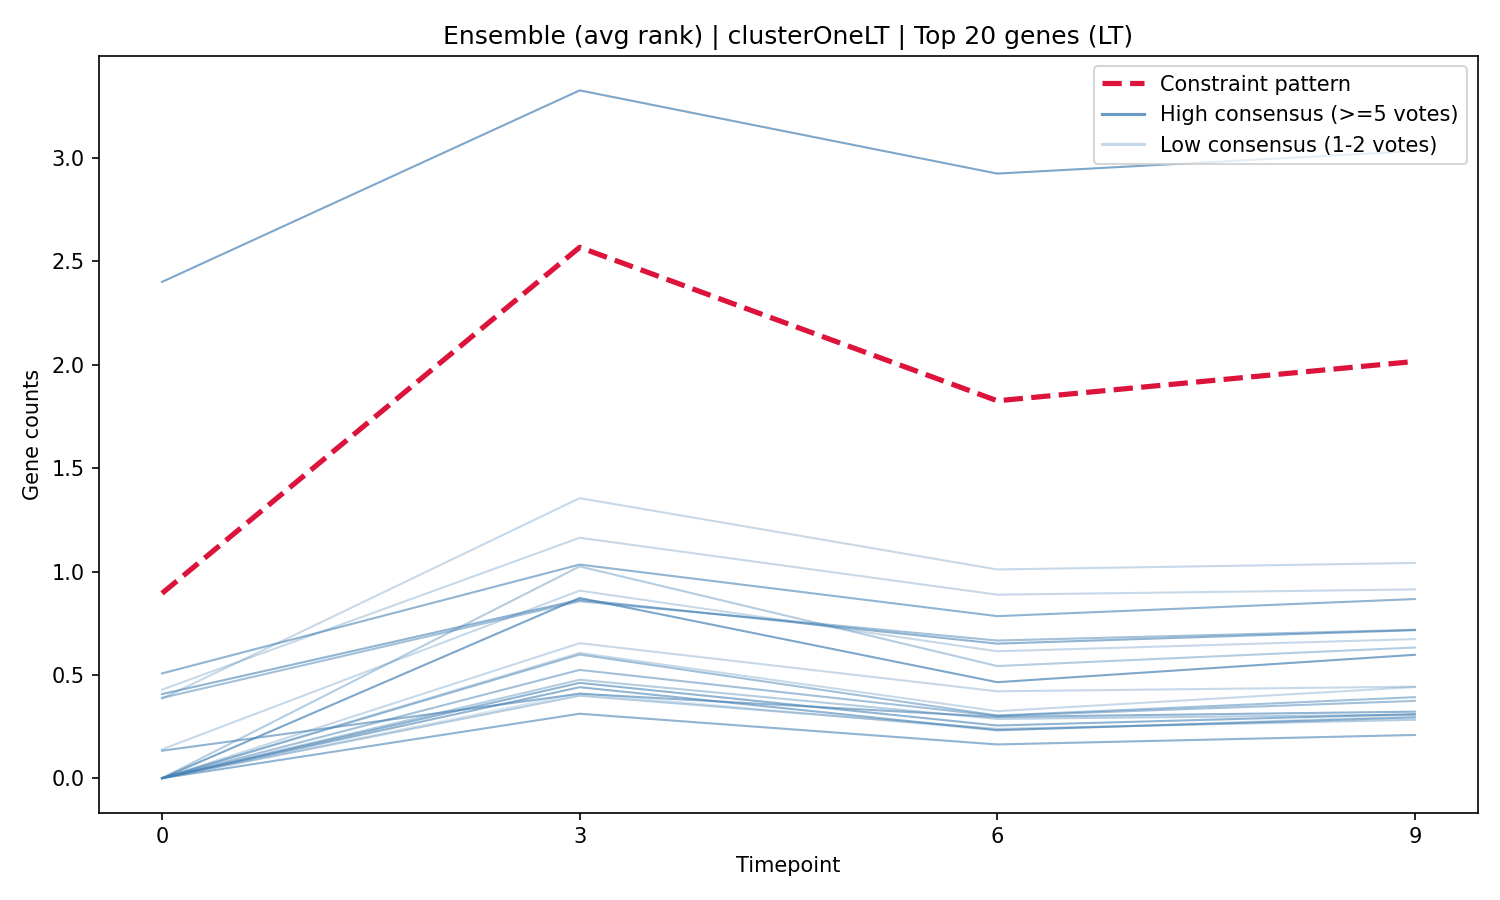
\includegraphics[height=0.85\textheight]{plots/Ensemble_LT_clusterOneLT_constraint.png}
\end{frame}

\begin{frame}{clusterOne LT — Overlap Heatmap}
\centering
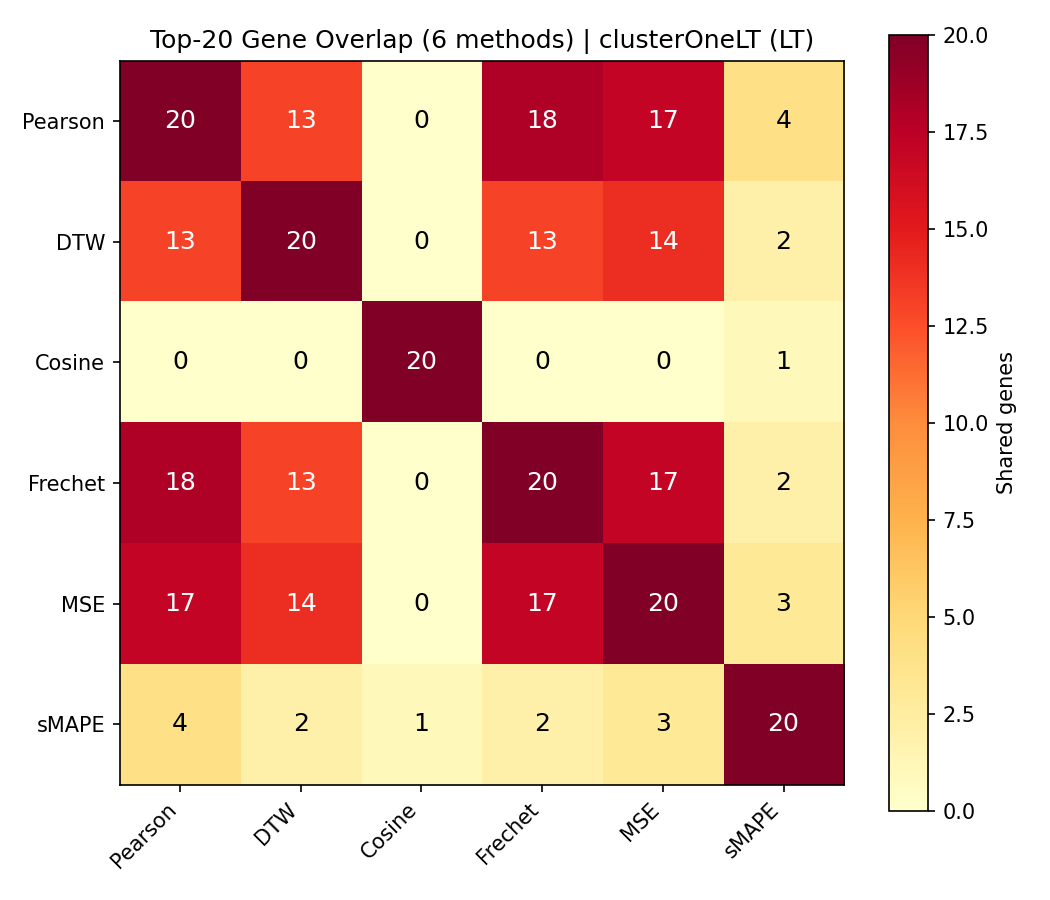
\includegraphics[height=0.85\textheight]{plots/overlap_6methods_LT_clusterOneLT.png}
\end{frame}

% --- clusterTwo LT ---
\begin{frame}{clusterTwo LT — Pearson}
\centering
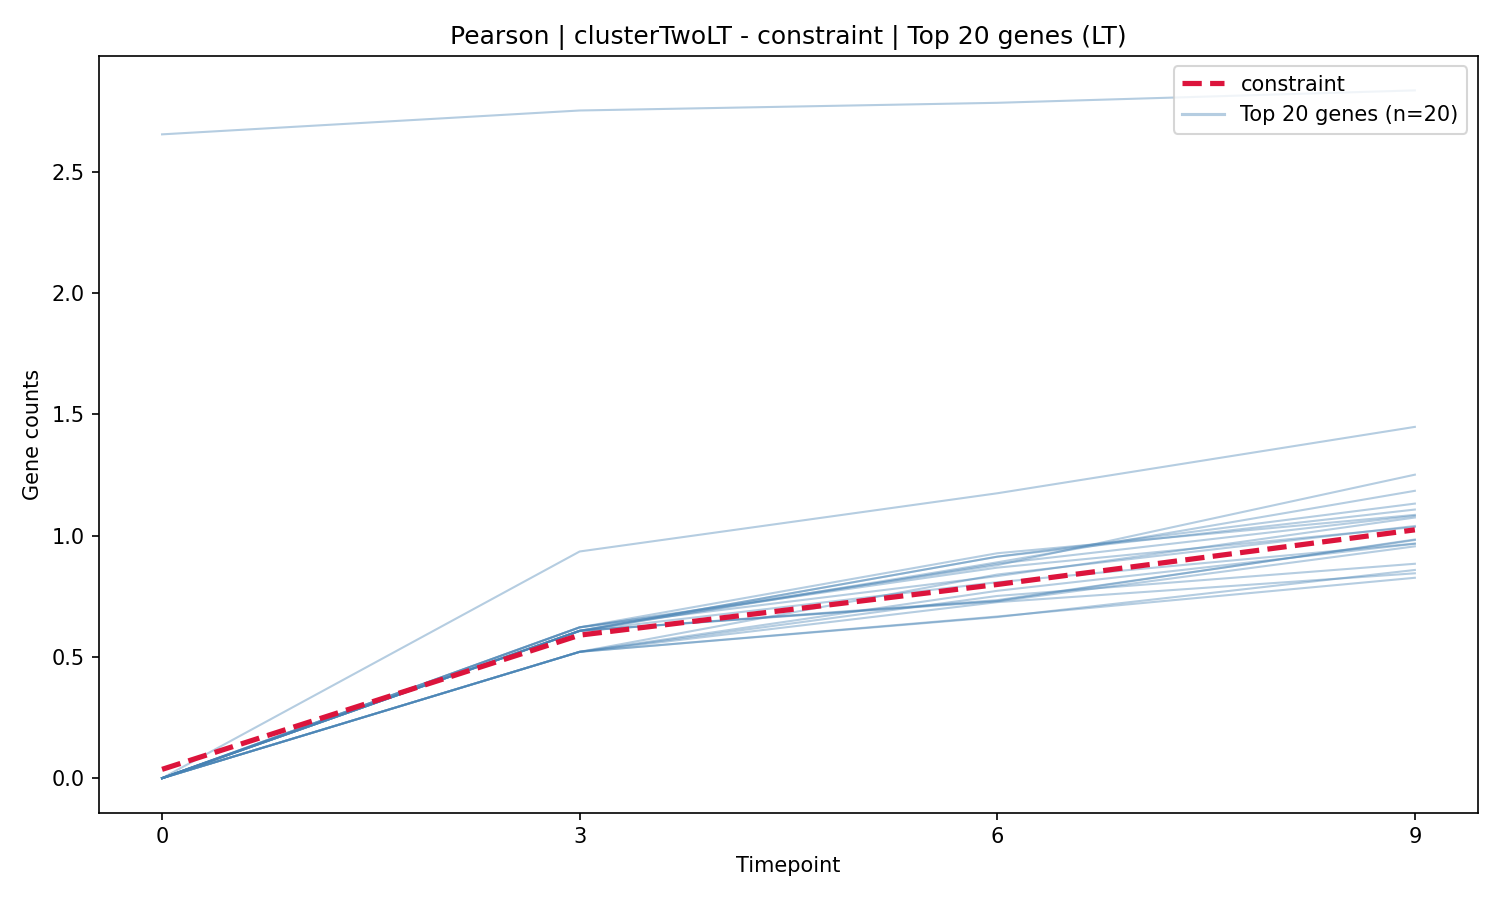
\includegraphics[height=0.85\textheight]{plots/Pearson_LT_clusterTwoLT_constraint.png}
\end{frame}

\begin{frame}{clusterTwo LT — DTW}
\centering
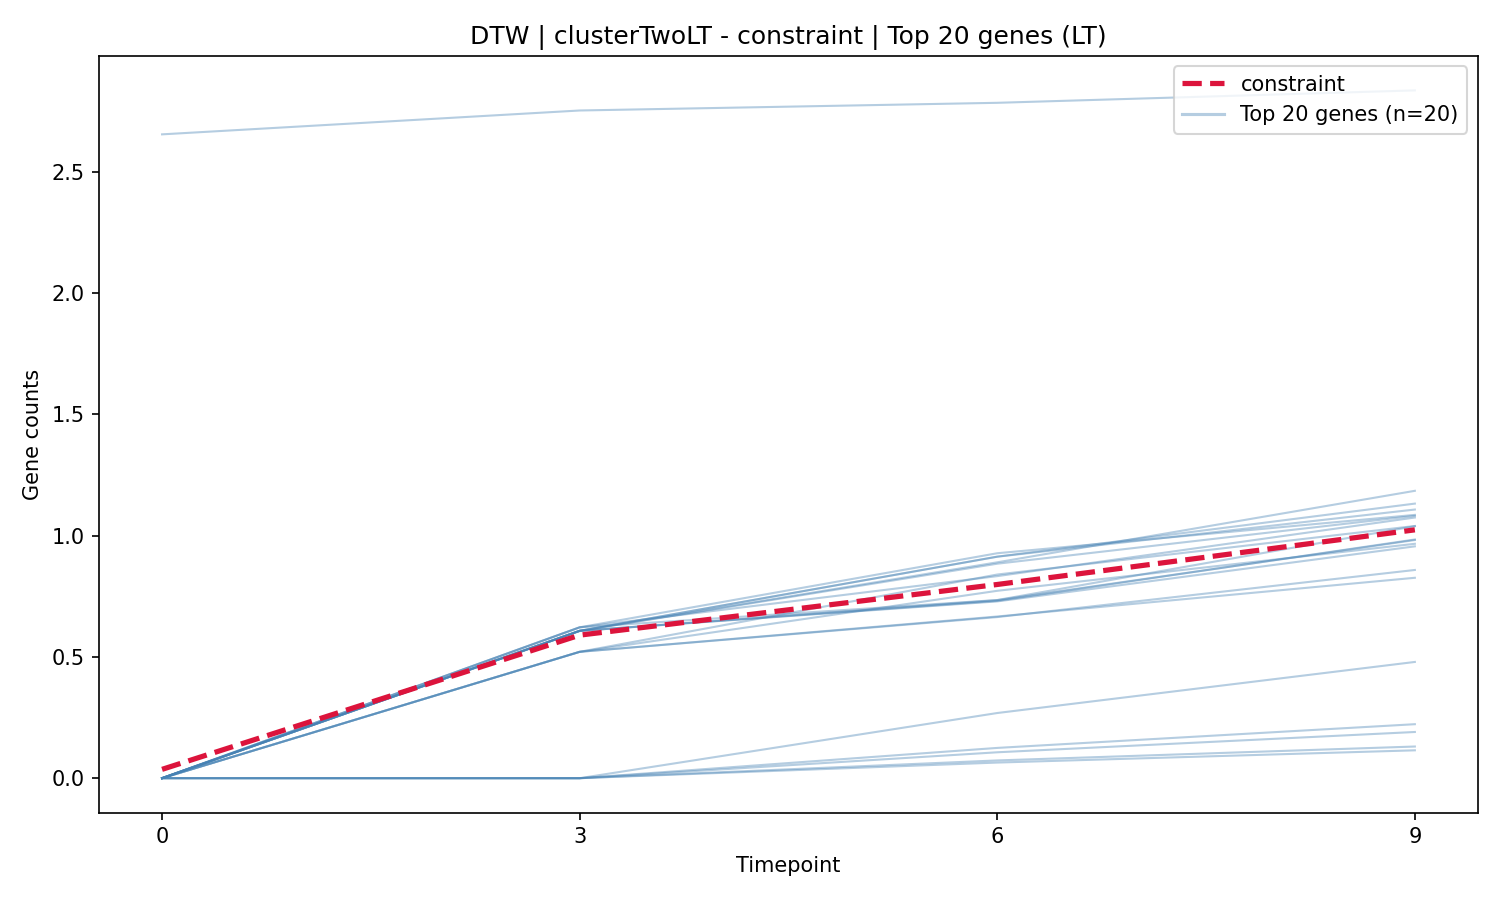
\includegraphics[height=0.85\textheight]{plots/DTW_LT_clusterTwoLT_constraint.png}
\end{frame}

\begin{frame}{clusterTwo LT — Cosine}
\centering
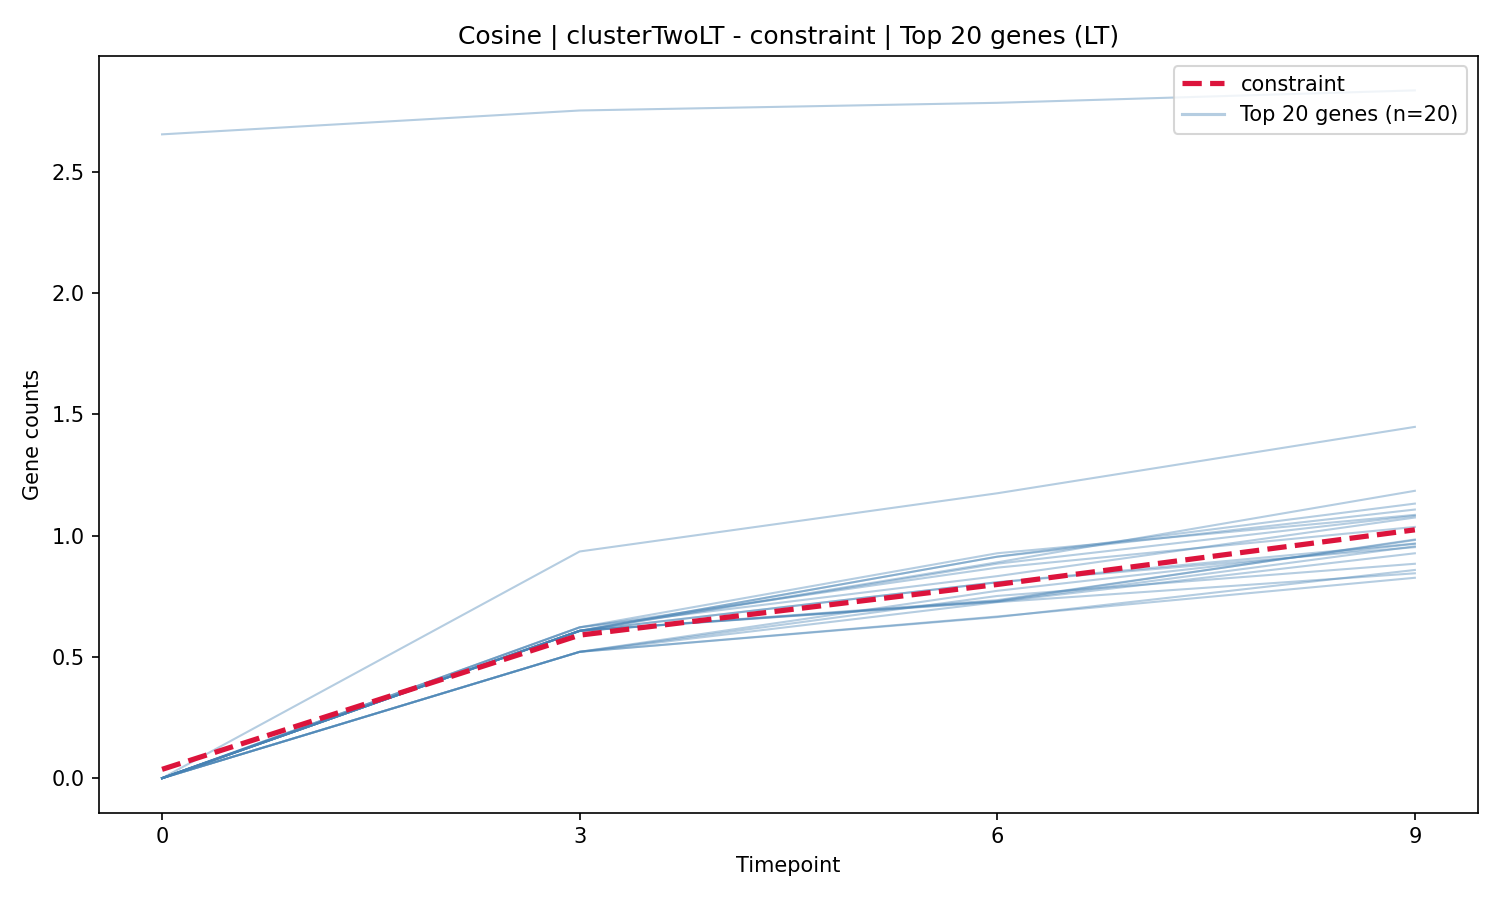
\includegraphics[height=0.85\textheight]{plots/Cosine_LT_clusterTwoLT_constraint.png}
\end{frame}

\begin{frame}{clusterTwo LT — Fr\'{e}chet}
\centering
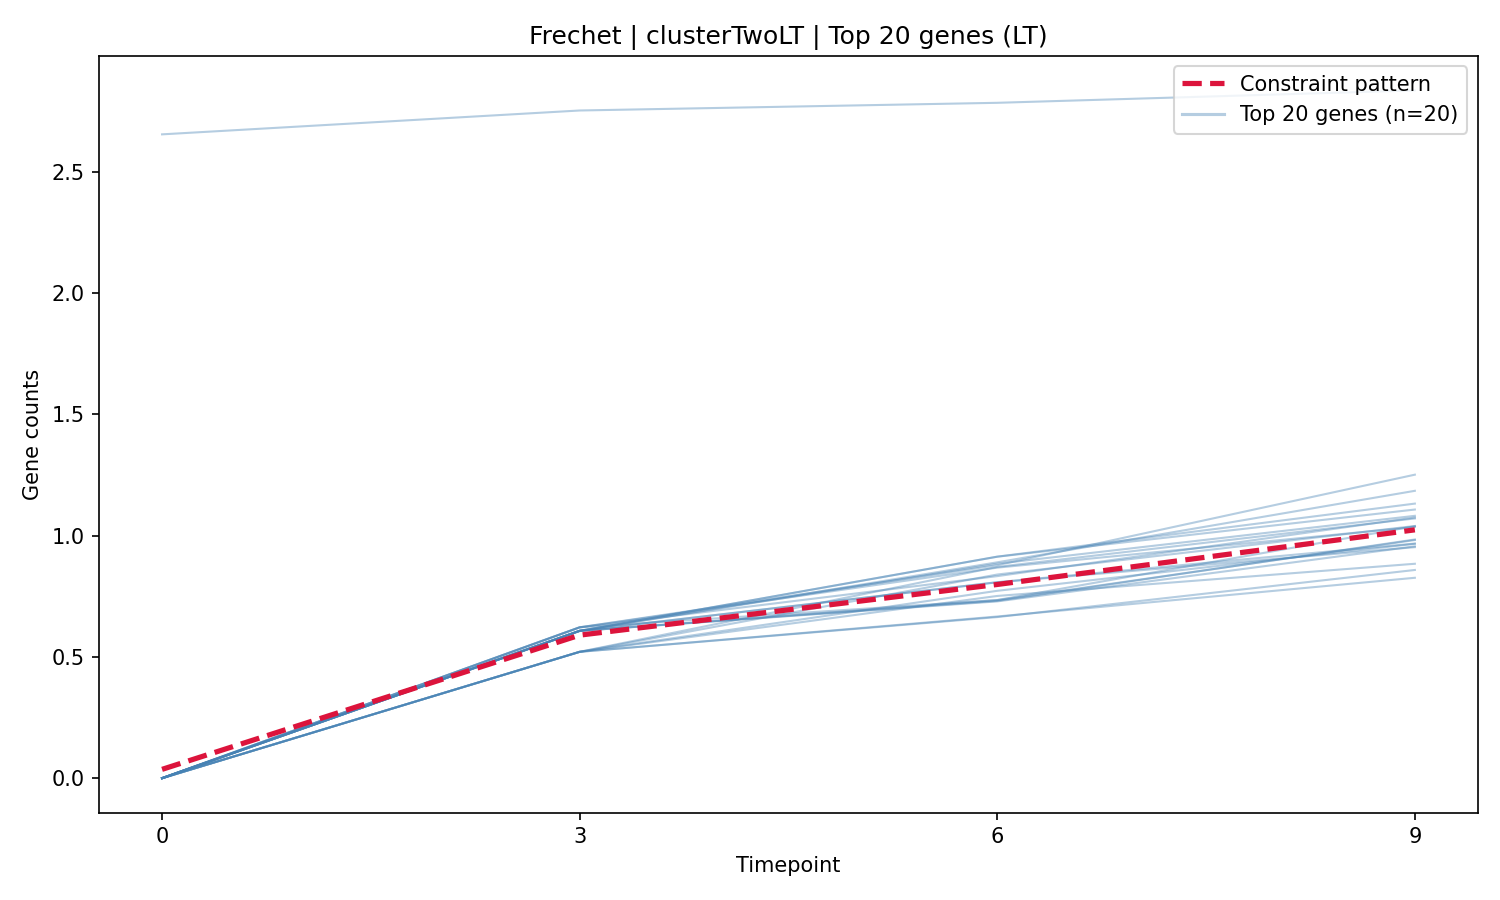
\includegraphics[height=0.85\textheight]{plots/Frechet_LT_clusterTwoLT_constraint.png}
\end{frame}

\begin{frame}{clusterTwo LT — MSE}
\centering
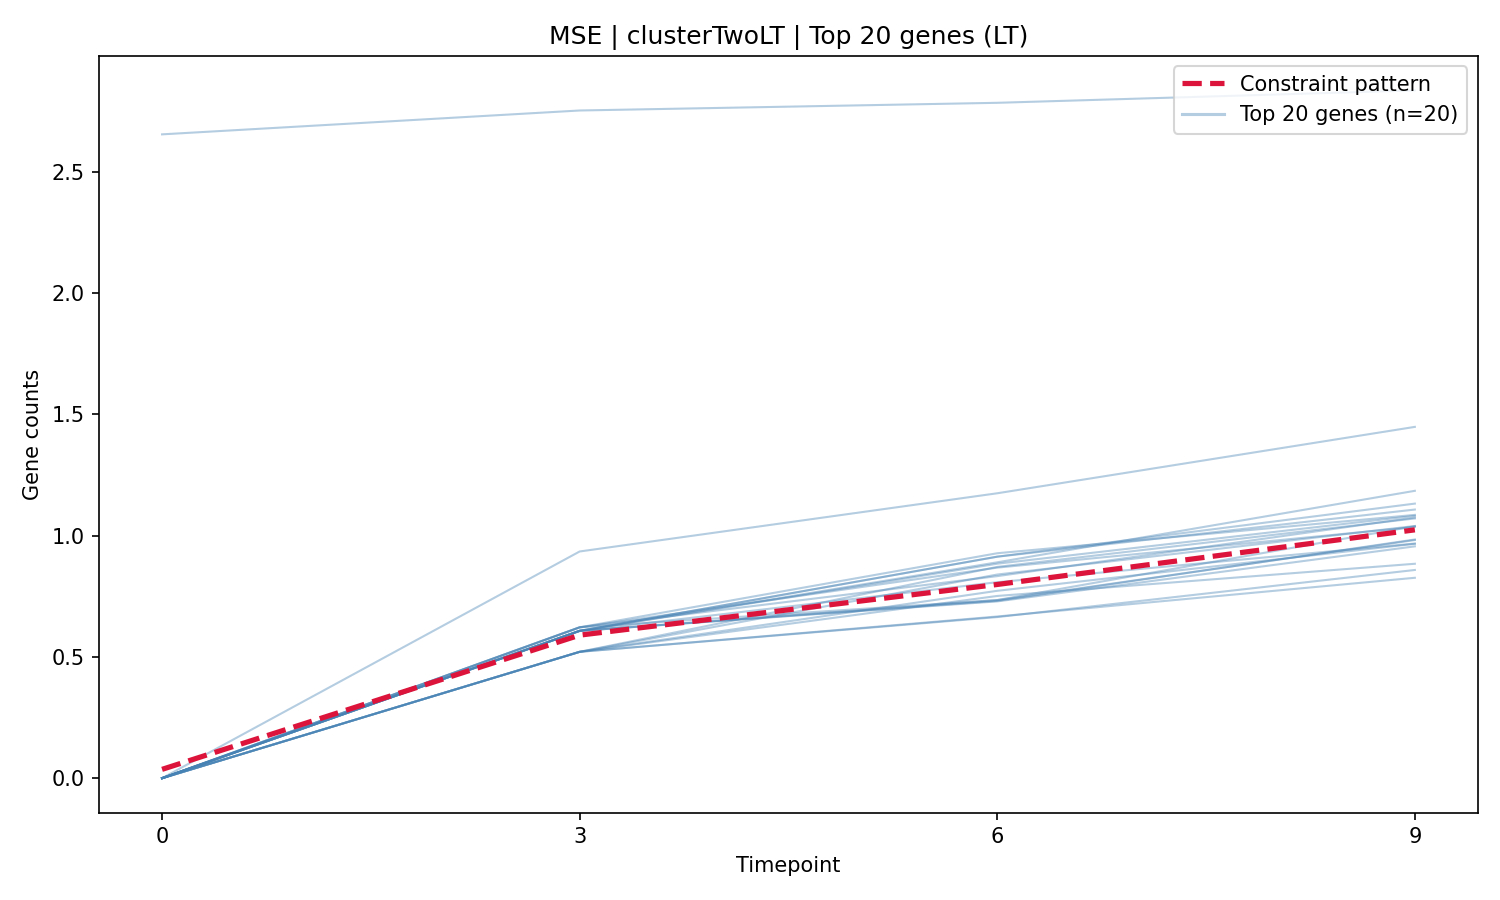
\includegraphics[height=0.85\textheight]{plots/MSE_LT_clusterTwoLT_constraint.png}
\end{frame}

\begin{frame}{clusterTwo LT — sMAPE}
\centering
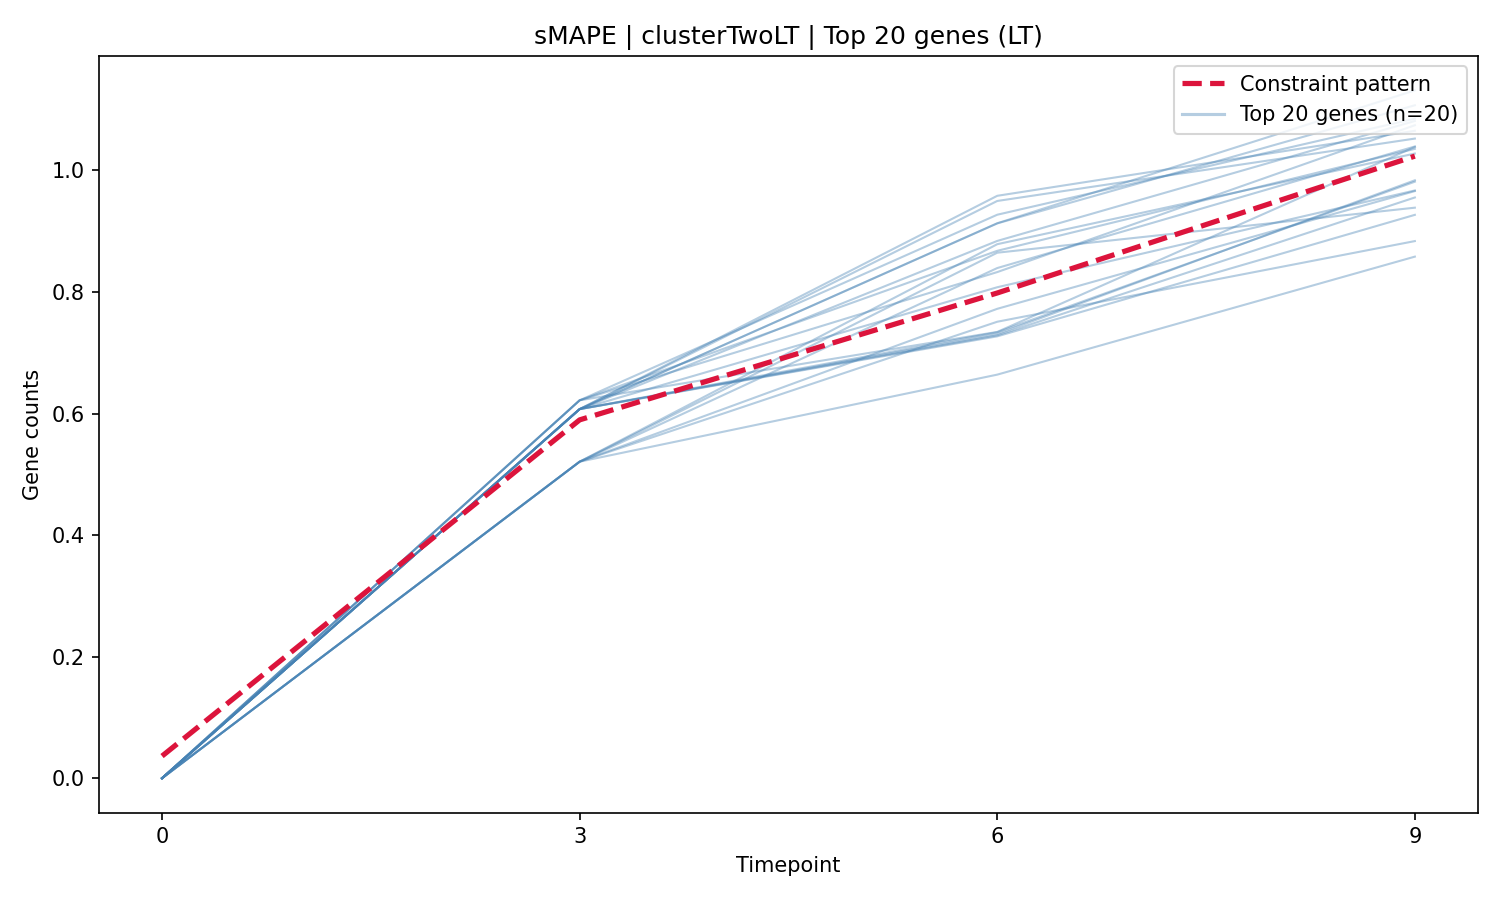
\includegraphics[height=0.85\textheight]{plots/sMAPE_LT_clusterTwoLT_constraint.png}
\end{frame}

\begin{frame}{clusterTwo LT — Ensemble}
\centering
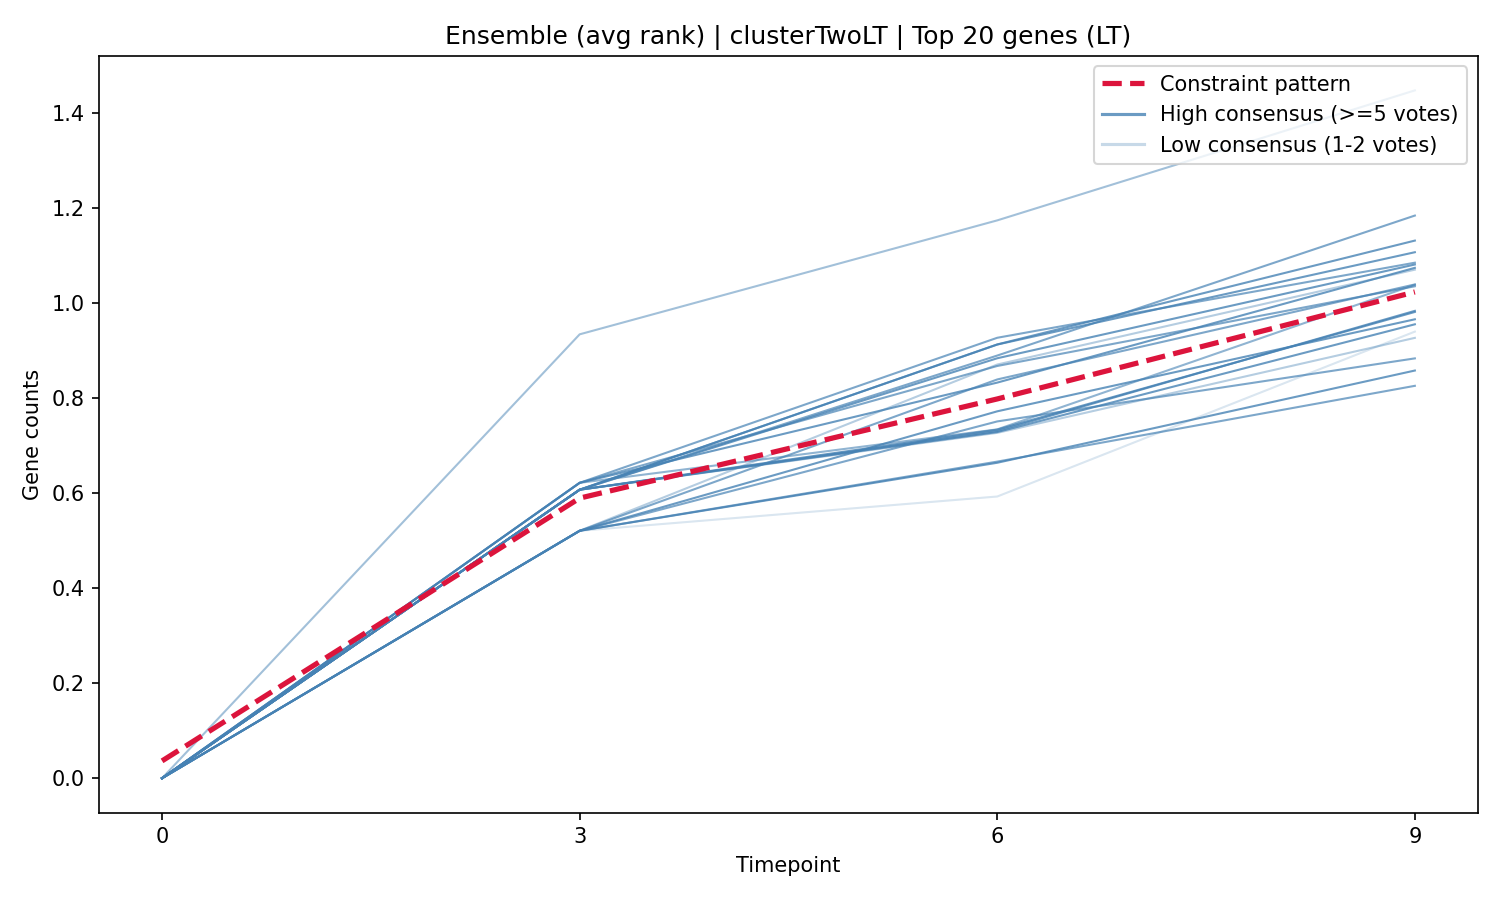
\includegraphics[height=0.85\textheight]{plots/Ensemble_LT_clusterTwoLT_constraint.png}
\end{frame}

\begin{frame}{clusterTwo LT — Overlap Heatmap}
\centering
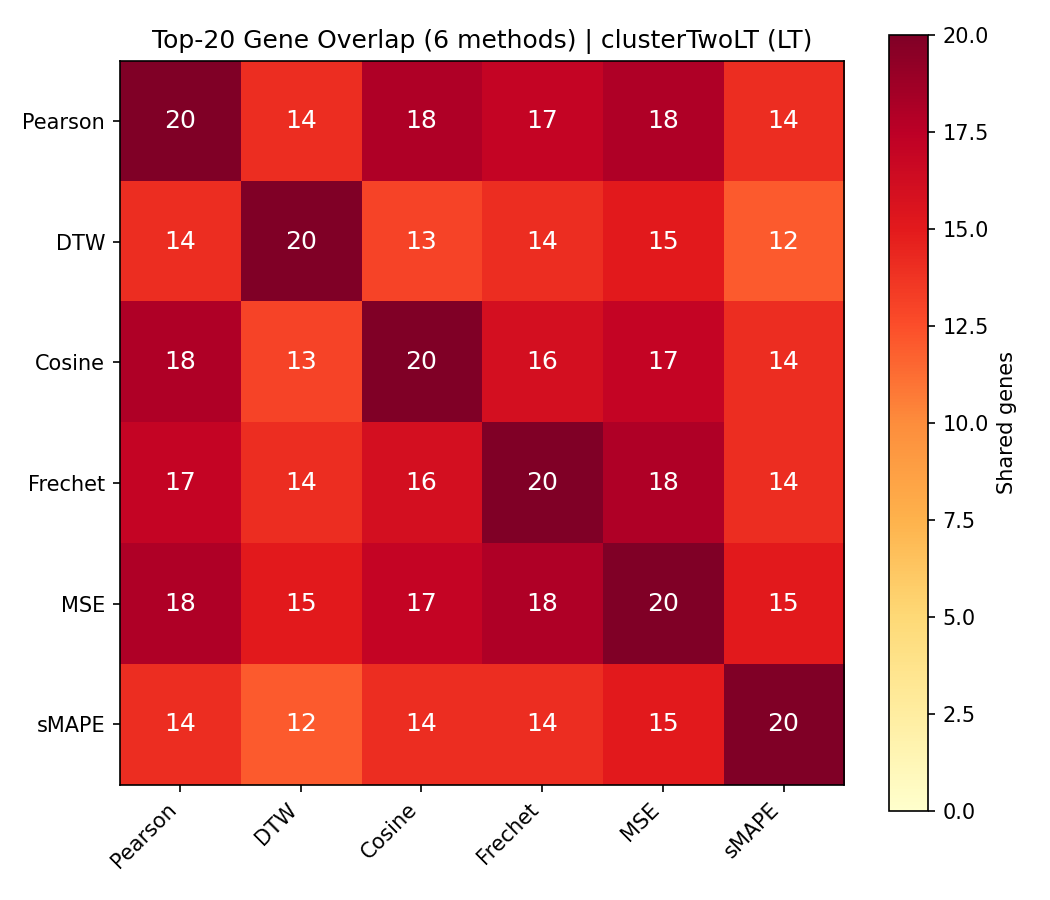
\includegraphics[height=0.85\textheight]{plots/overlap_6methods_LT_clusterTwoLT.png}
\end{frame}

% --- clusterThree LT ---
\begin{frame}{clusterThree LT — Pearson}
\centering
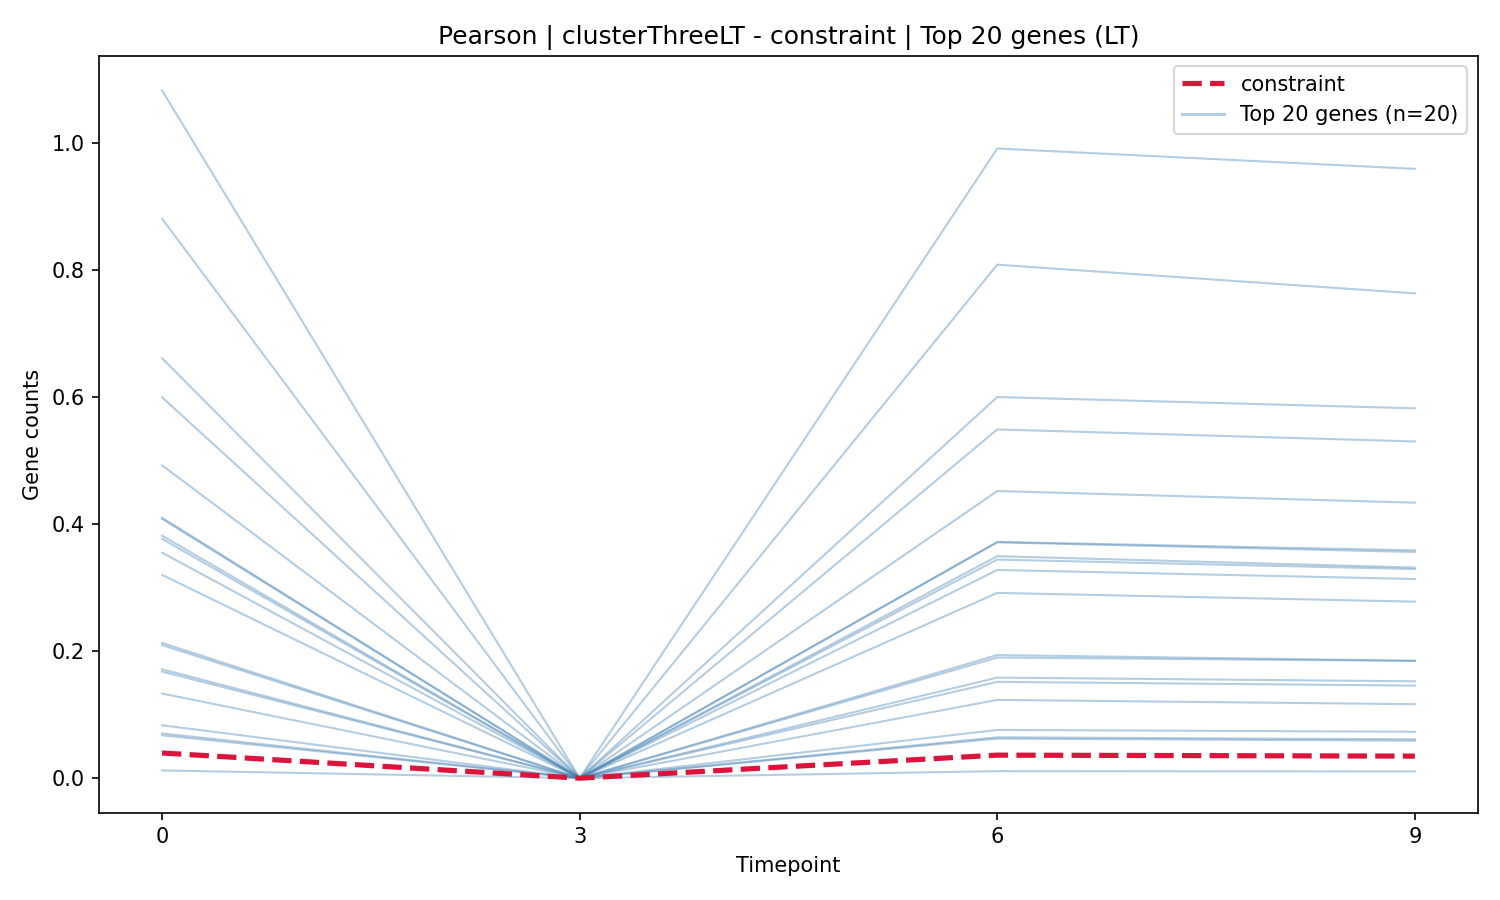
\includegraphics[height=0.85\textheight]{plots/Pearson_LT_clusterThreeLT_constraint.png}
\end{frame}

\begin{frame}{clusterThree LT — DTW}
\centering
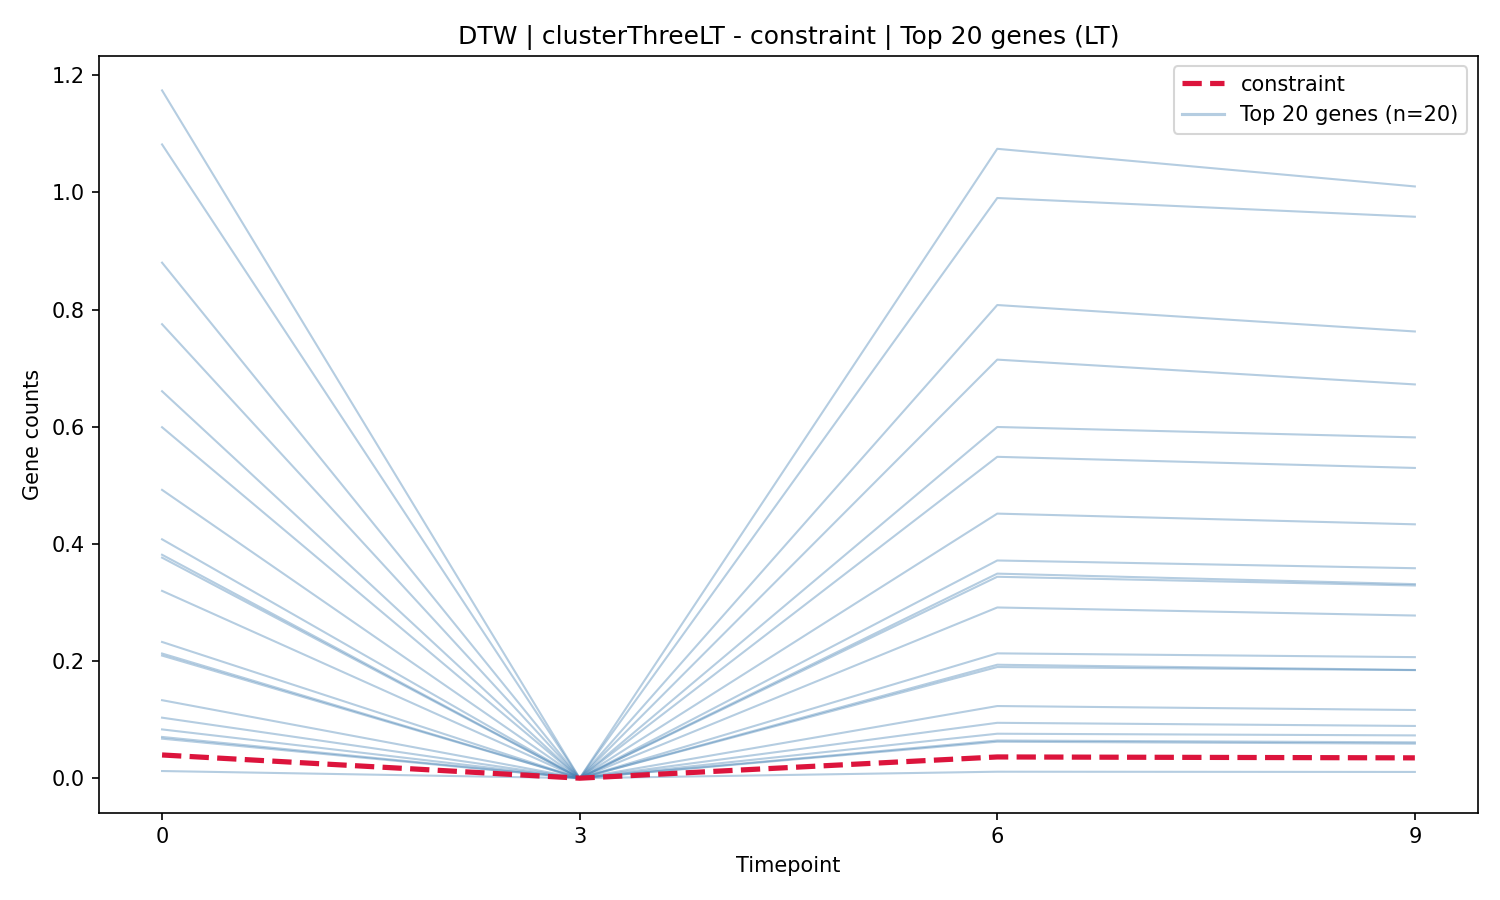
\includegraphics[height=0.85\textheight]{plots/DTW_LT_clusterThreeLT_constraint.png}
\end{frame}

\begin{frame}{clusterThree LT — Cosine}
\centering
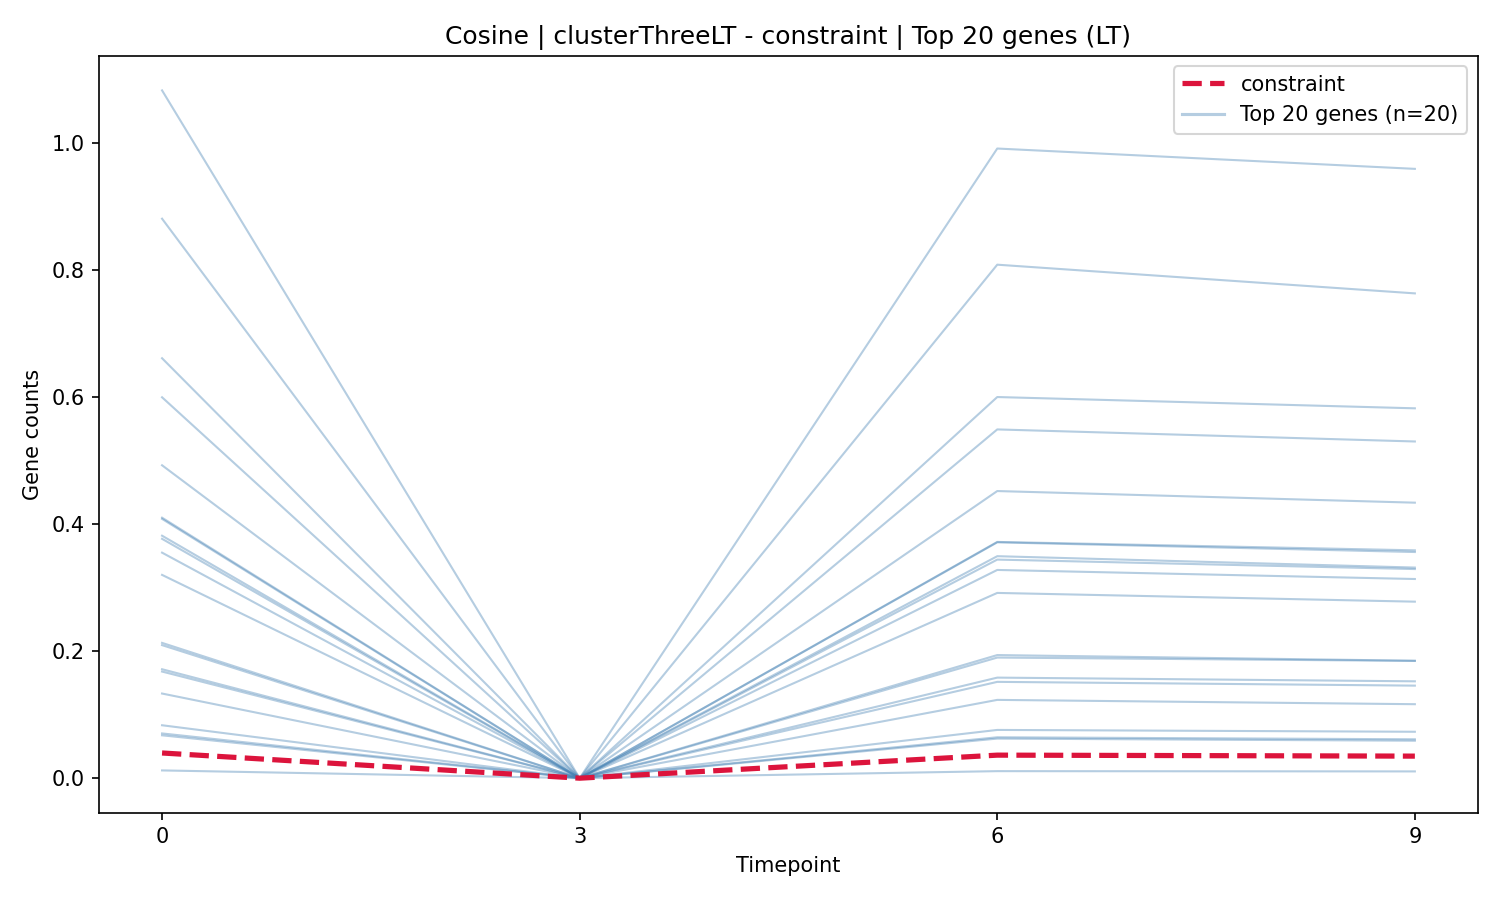
\includegraphics[height=0.85\textheight]{plots/Cosine_LT_clusterThreeLT_constraint.png}
\end{frame}

\begin{frame}{clusterThree LT — Fr\'{e}chet}
\centering
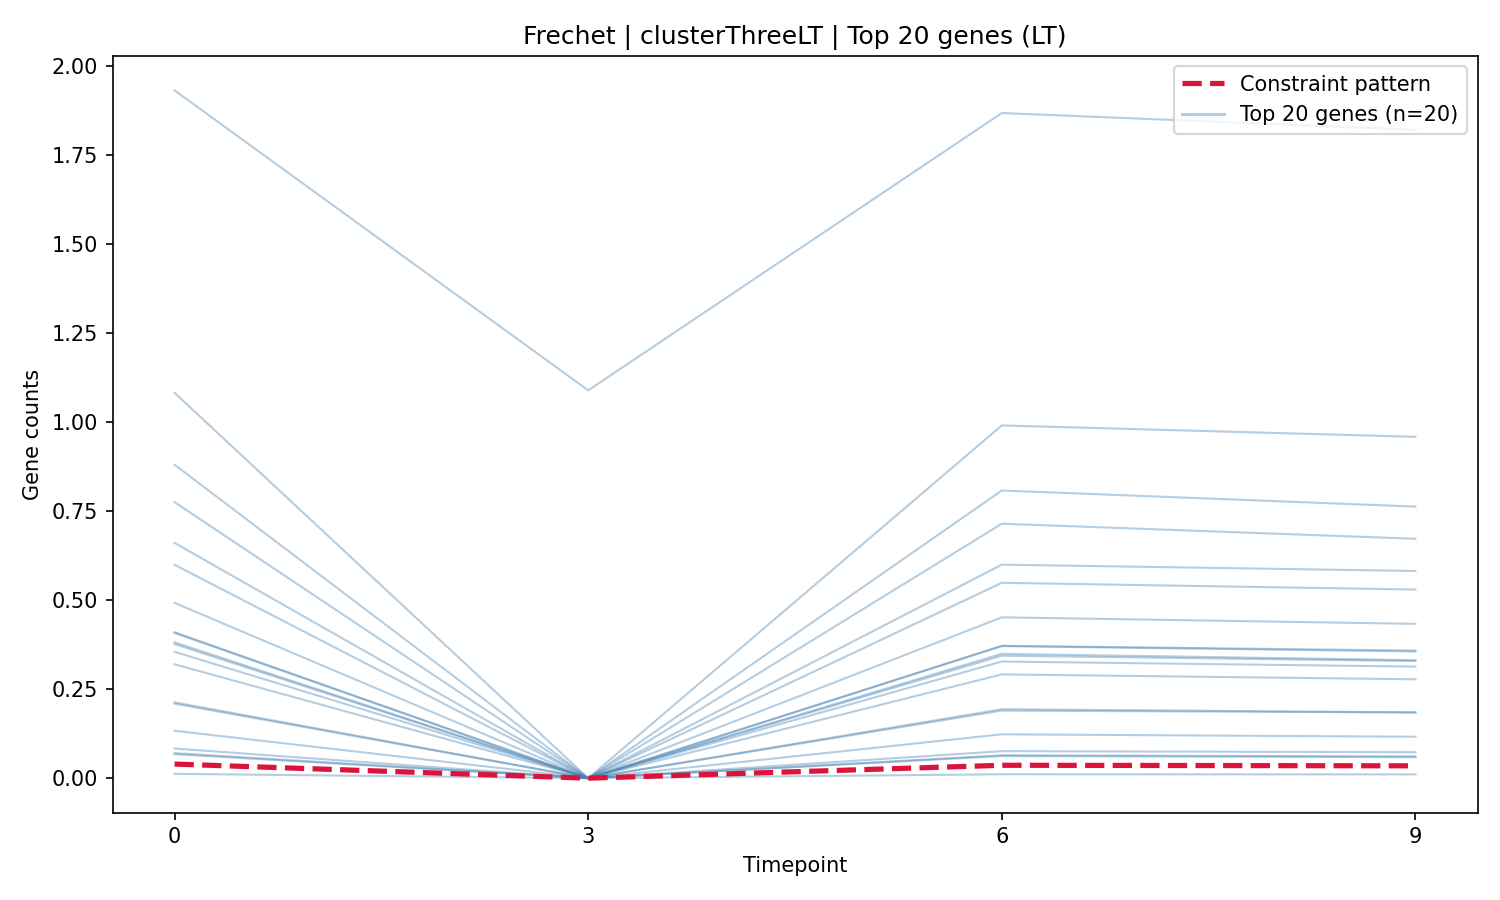
\includegraphics[height=0.85\textheight]{plots/Frechet_LT_clusterThreeLT_constraint.png}
\end{frame}

\begin{frame}{clusterThree LT — MSE}
\centering
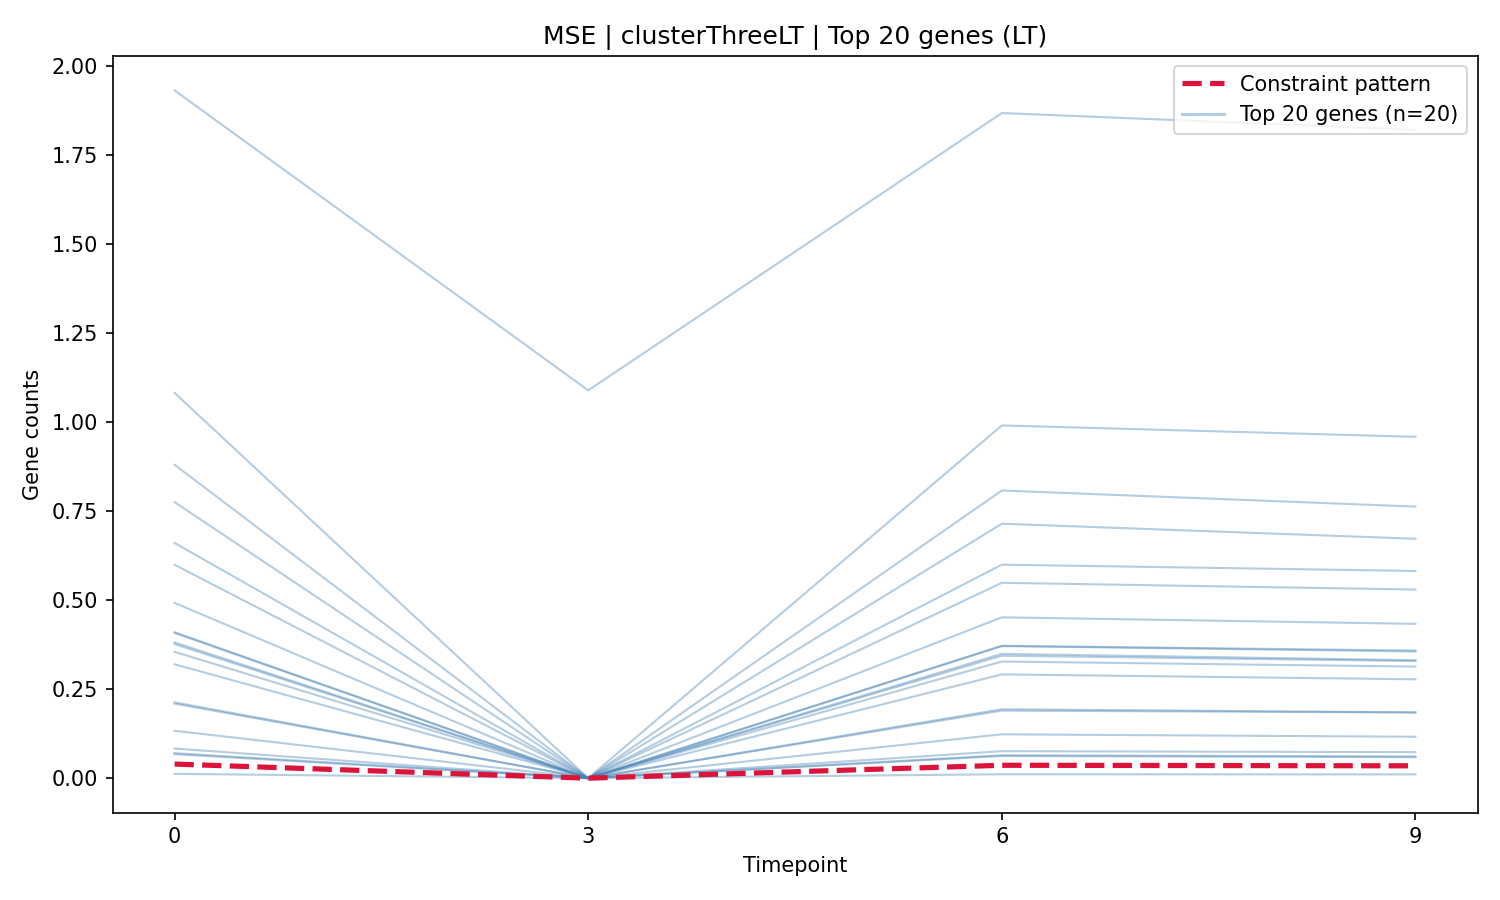
\includegraphics[height=0.85\textheight]{plots/MSE_LT_clusterThreeLT_constraint.png}
\end{frame}

\begin{frame}{clusterThree LT — sMAPE}
\centering
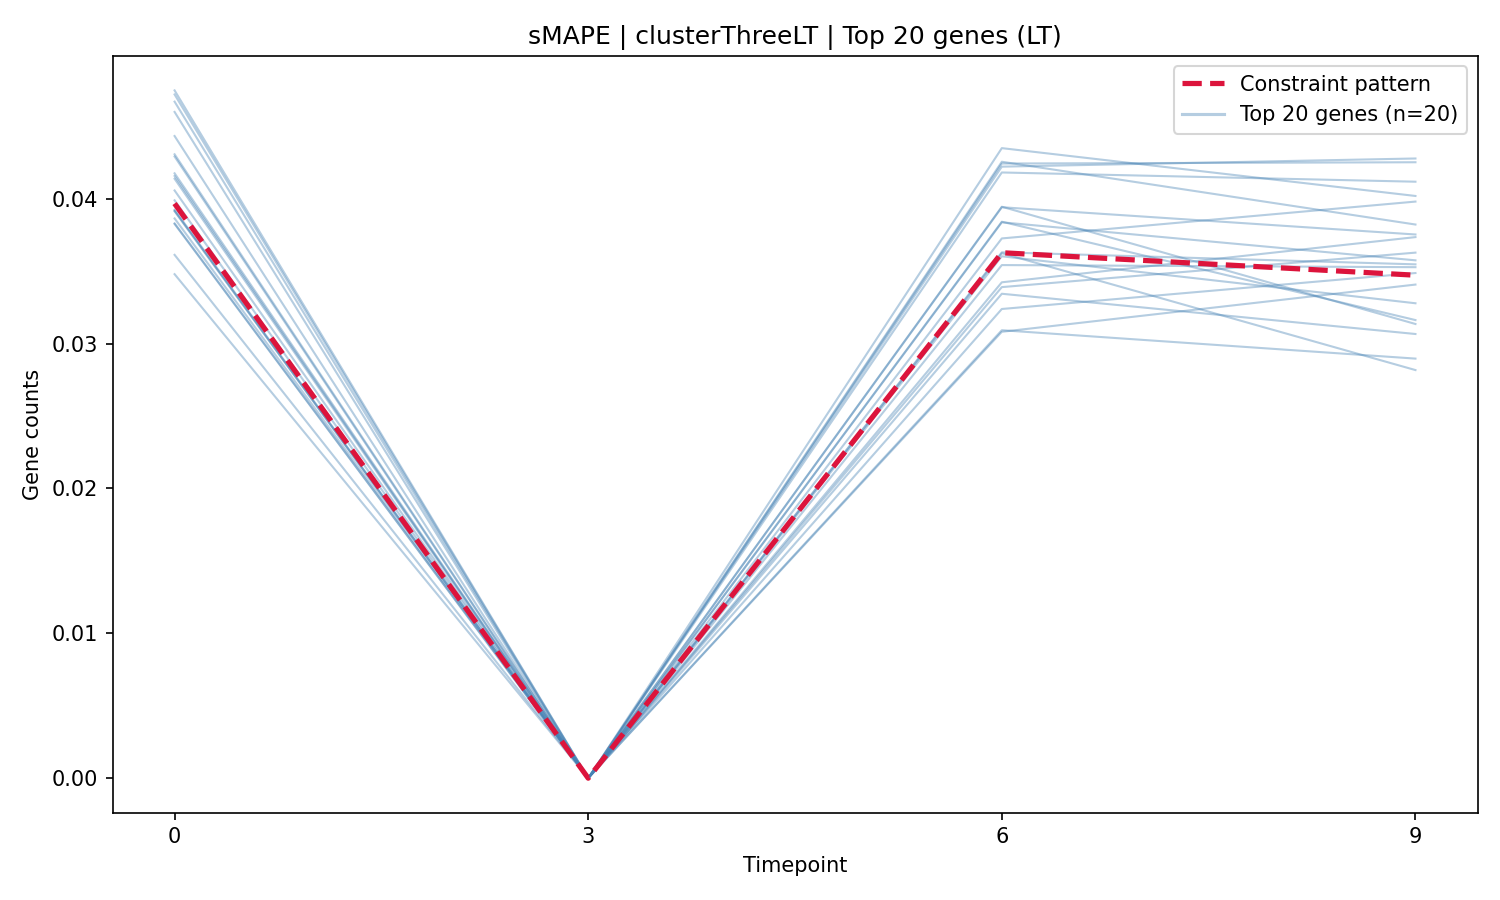
\includegraphics[height=0.85\textheight]{plots/sMAPE_LT_clusterThreeLT_constraint.png}
\end{frame}

\begin{frame}{clusterThree LT — Ensemble}
\centering
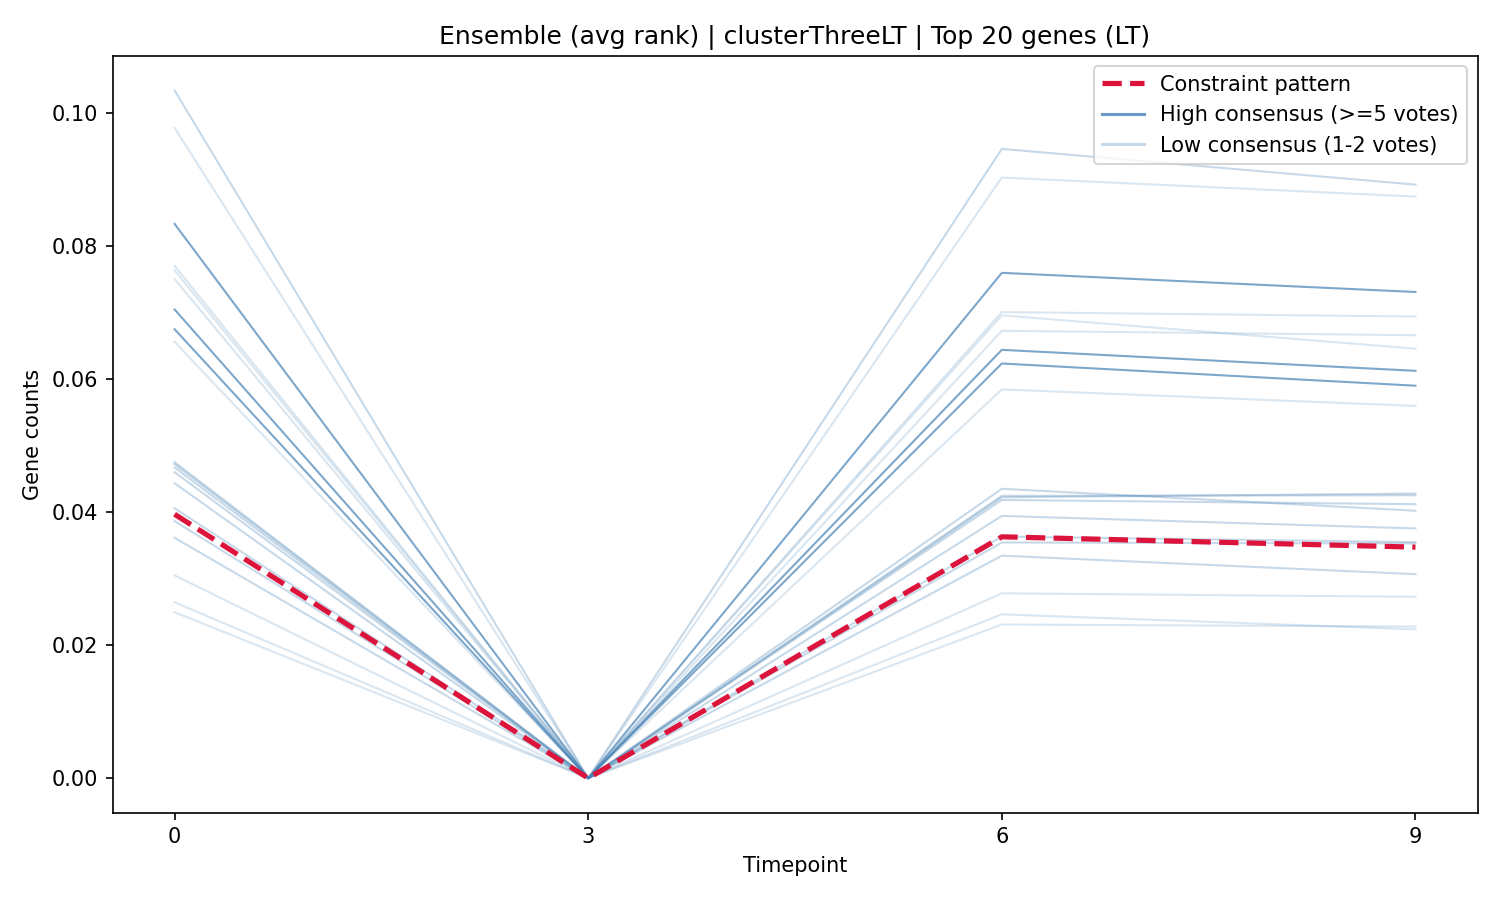
\includegraphics[height=0.85\textheight]{plots/Ensemble_LT_clusterThreeLT_constraint.png}
\end{frame}

\begin{frame}{clusterThree LT — Overlap Heatmap}
\centering
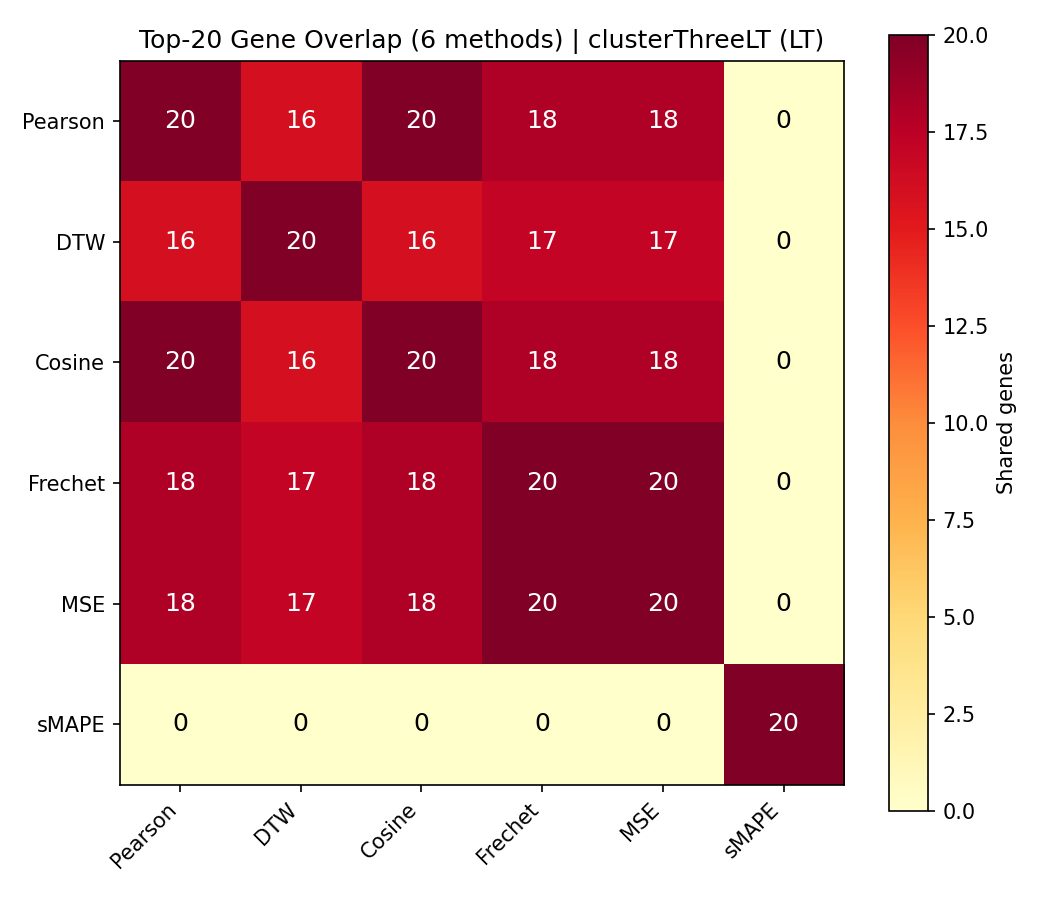
\includegraphics[height=0.85\textheight]{plots/overlap_6methods_LT_clusterThreeLT.png}
\end{frame}

% --- clusterFour LT ---
\begin{frame}{clusterFour LT — Pearson}
\centering
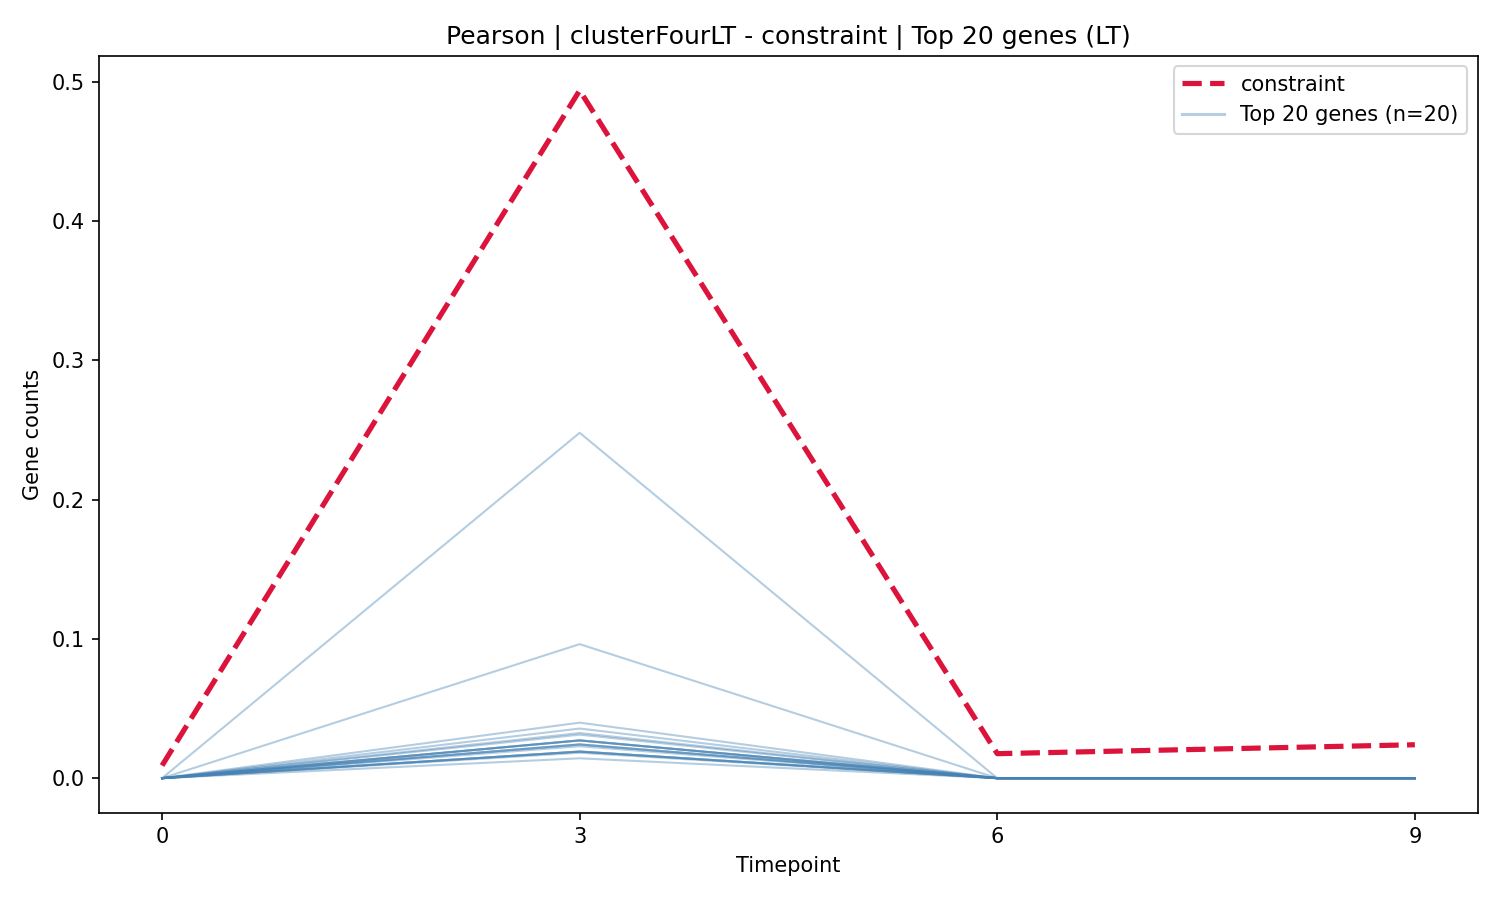
\includegraphics[height=0.85\textheight]{plots/Pearson_LT_clusterFourLT_constraint.png}
\end{frame}

\begin{frame}{clusterFour LT — DTW}
\centering
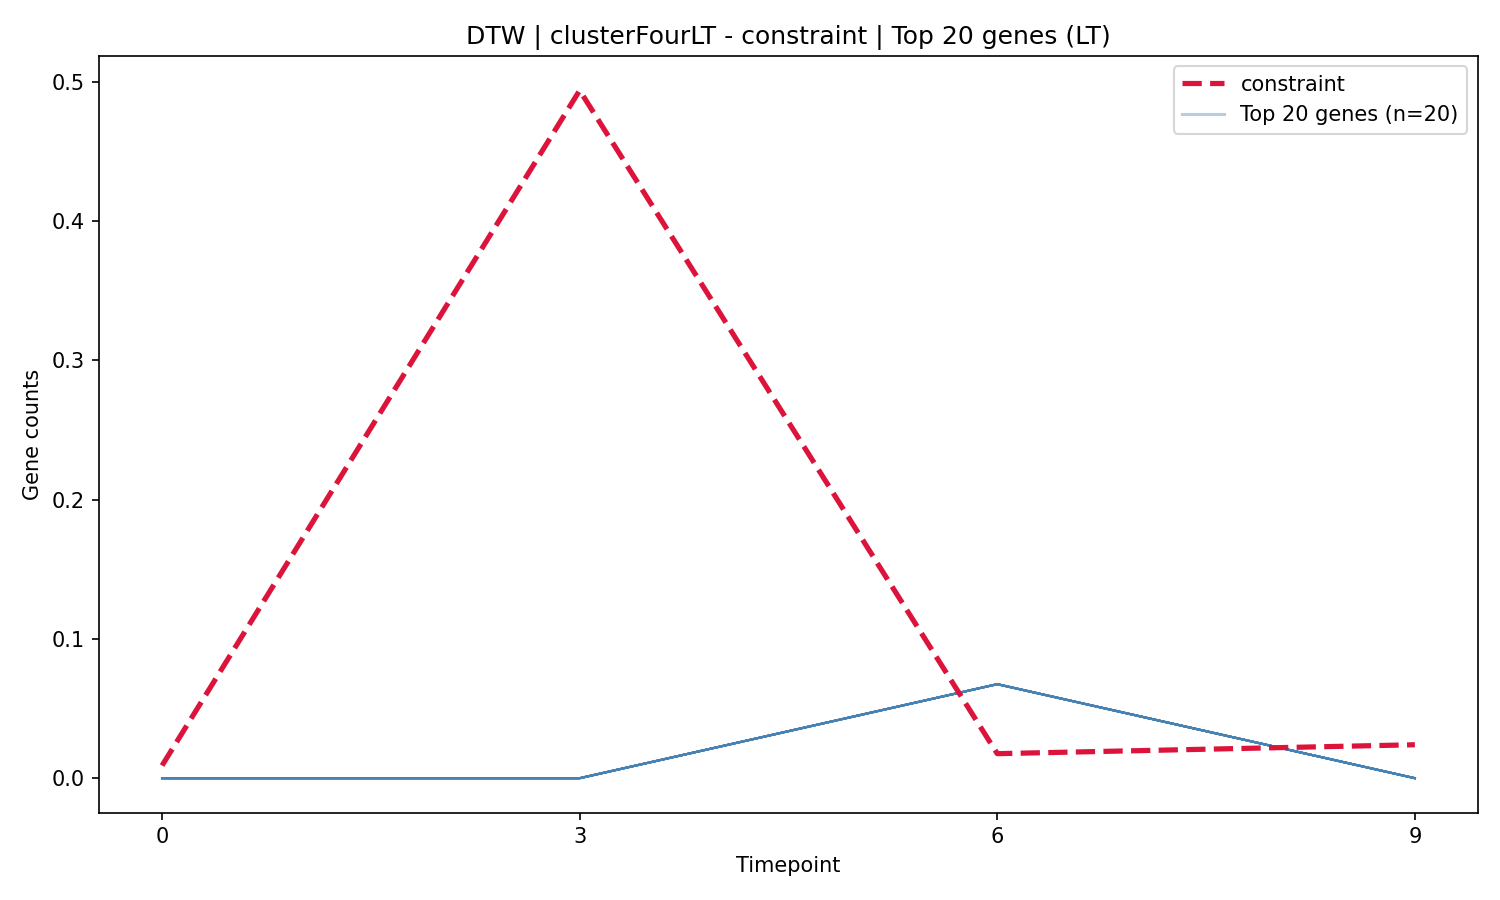
\includegraphics[height=0.85\textheight]{plots/DTW_LT_clusterFourLT_constraint.png}
\end{frame}

\begin{frame}{clusterFour LT — Cosine}
\centering
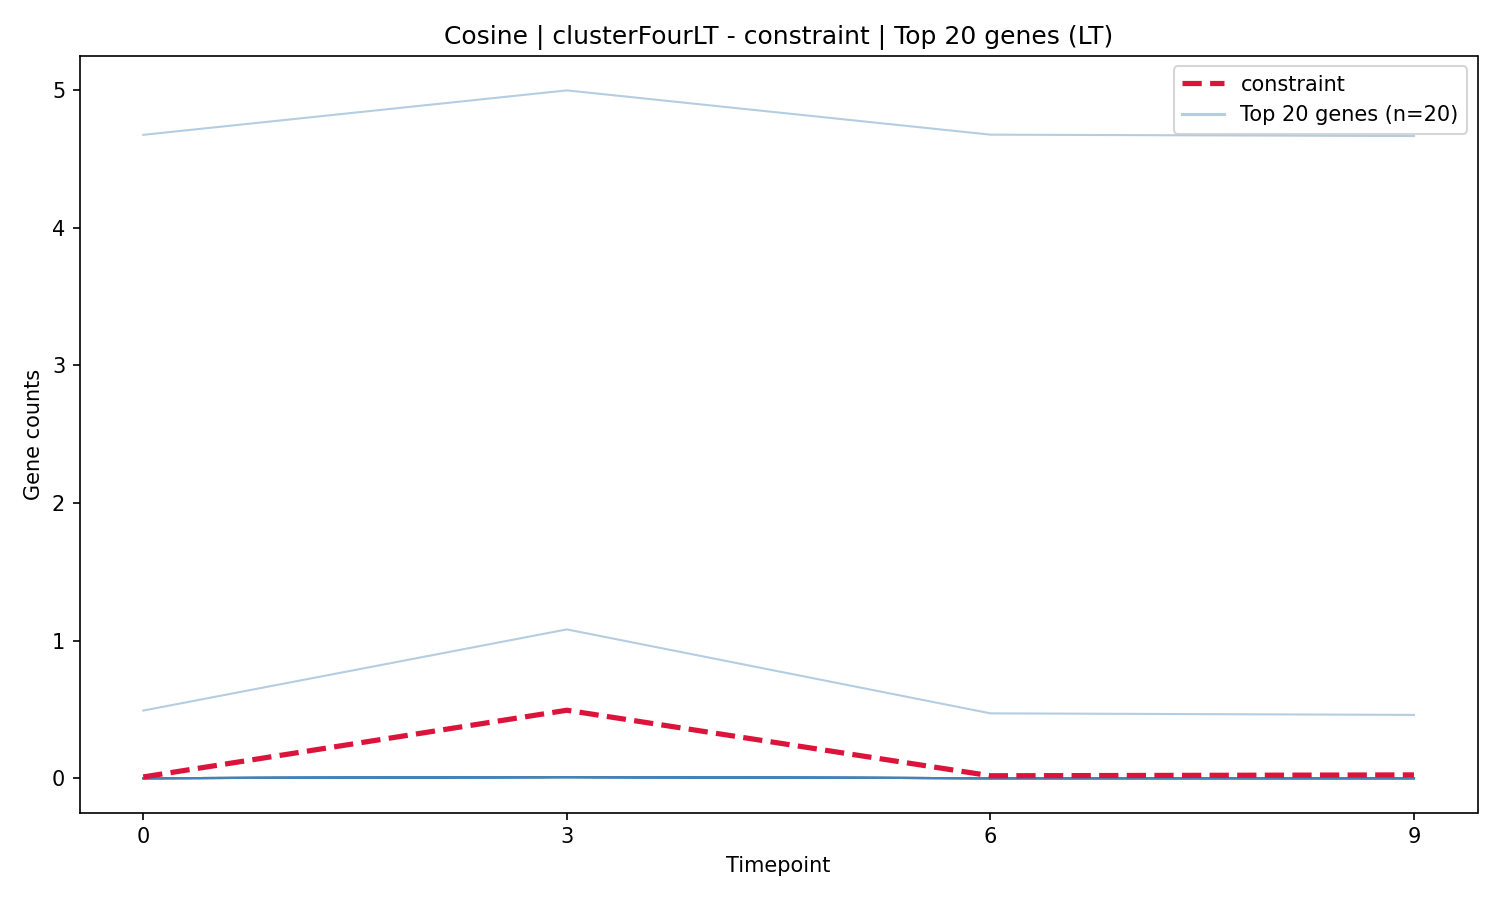
\includegraphics[height=0.85\textheight]{plots/Cosine_LT_clusterFourLT_constraint.png}
\end{frame}

\begin{frame}{clusterFour LT — Fr\'{e}chet}
\centering
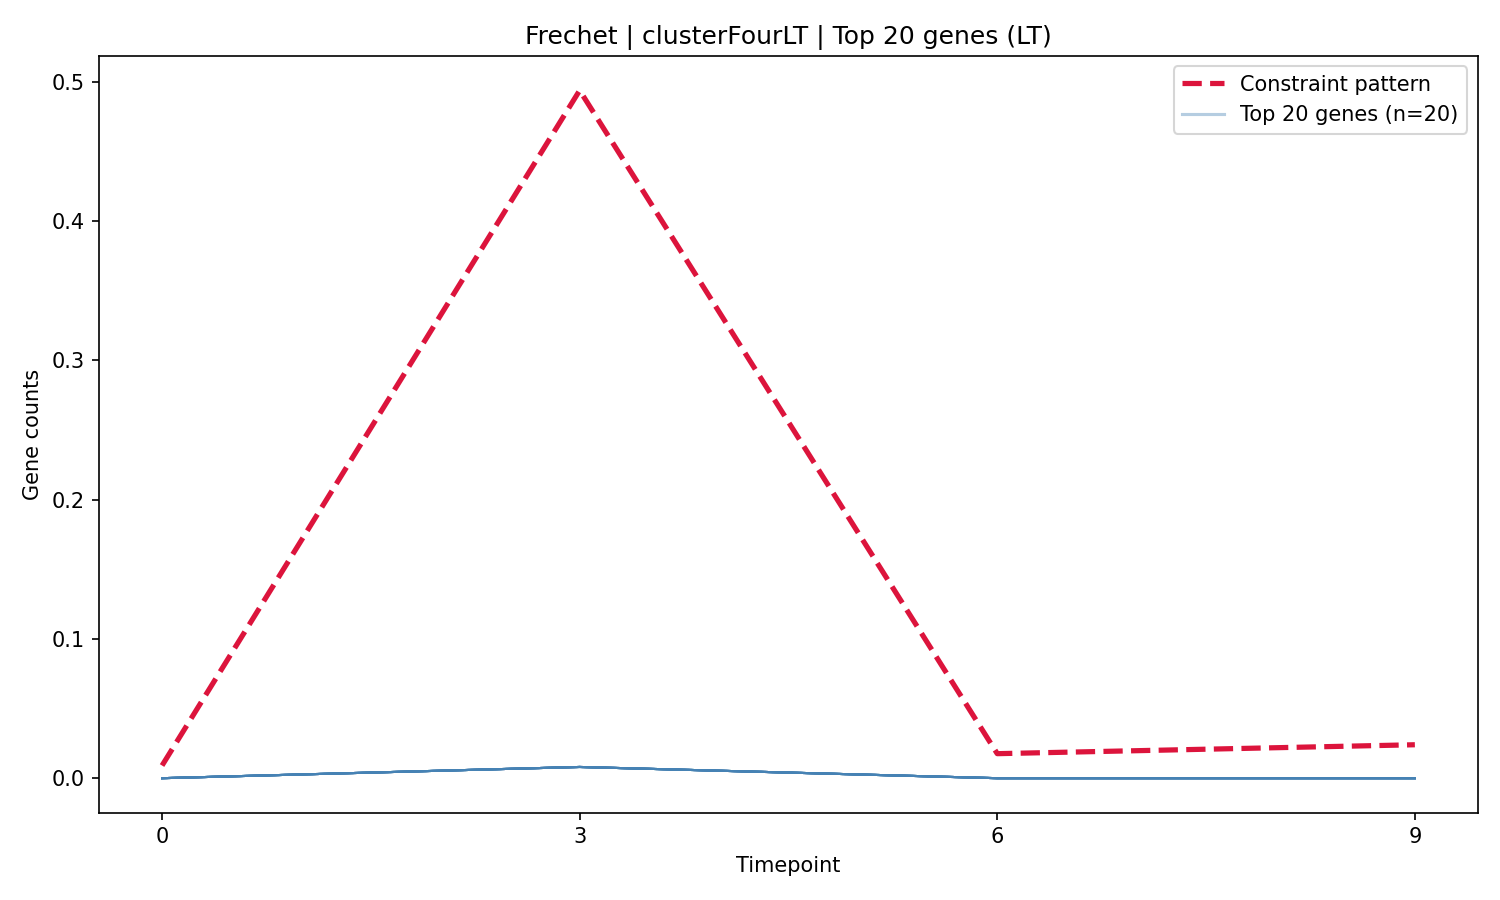
\includegraphics[height=0.85\textheight]{plots/Frechet_LT_clusterFourLT_constraint.png}
\end{frame}

\begin{frame}{clusterFour LT — MSE}
\centering
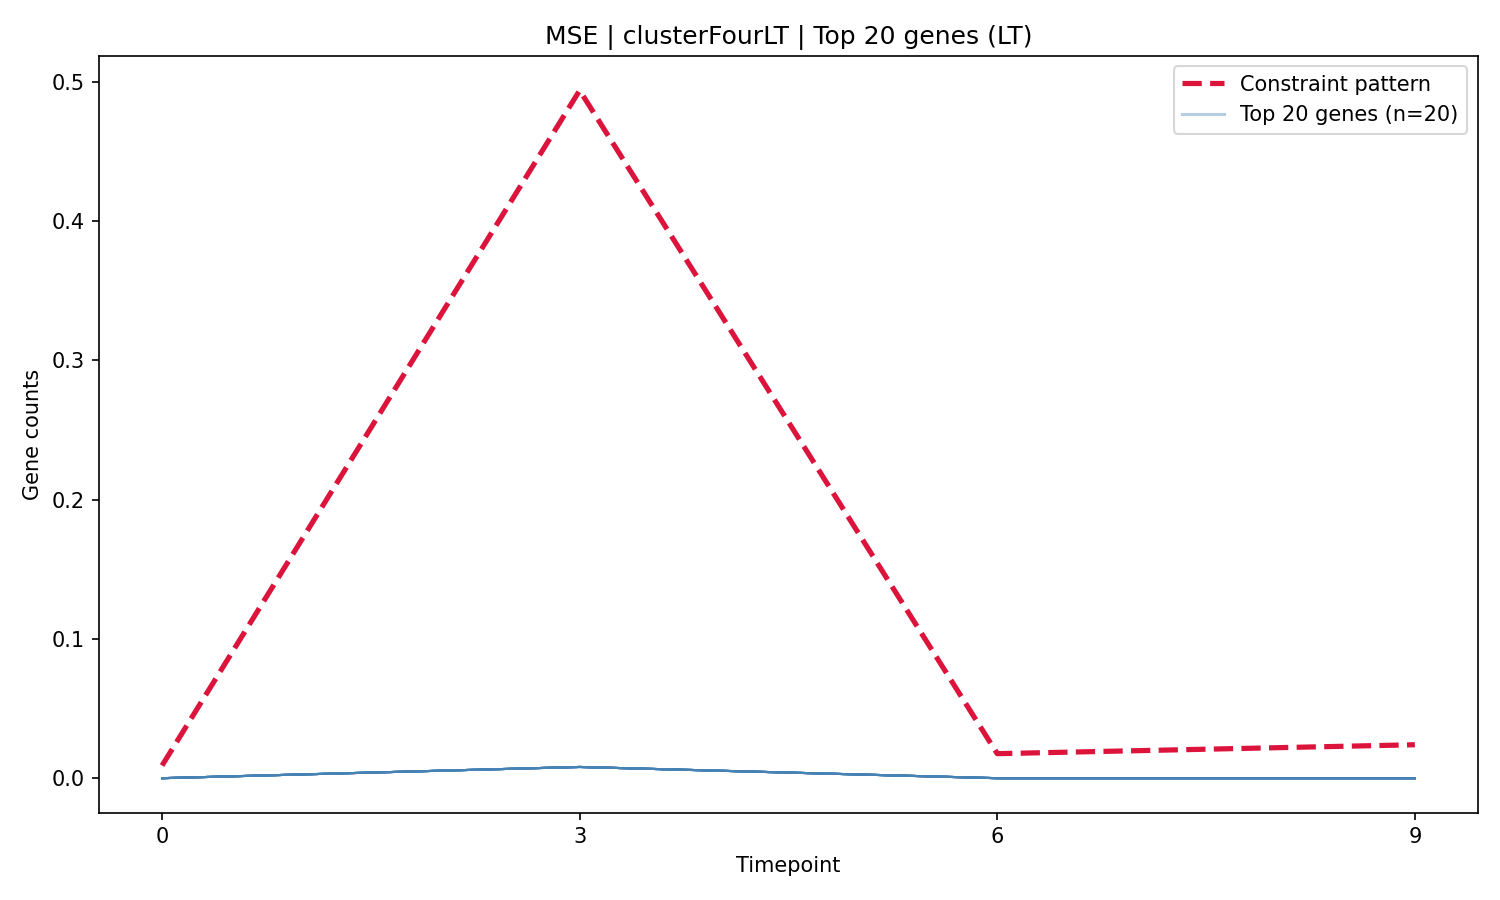
\includegraphics[height=0.85\textheight]{plots/MSE_LT_clusterFourLT_constraint.png}
\end{frame}

\begin{frame}{clusterFour LT — sMAPE}
\centering
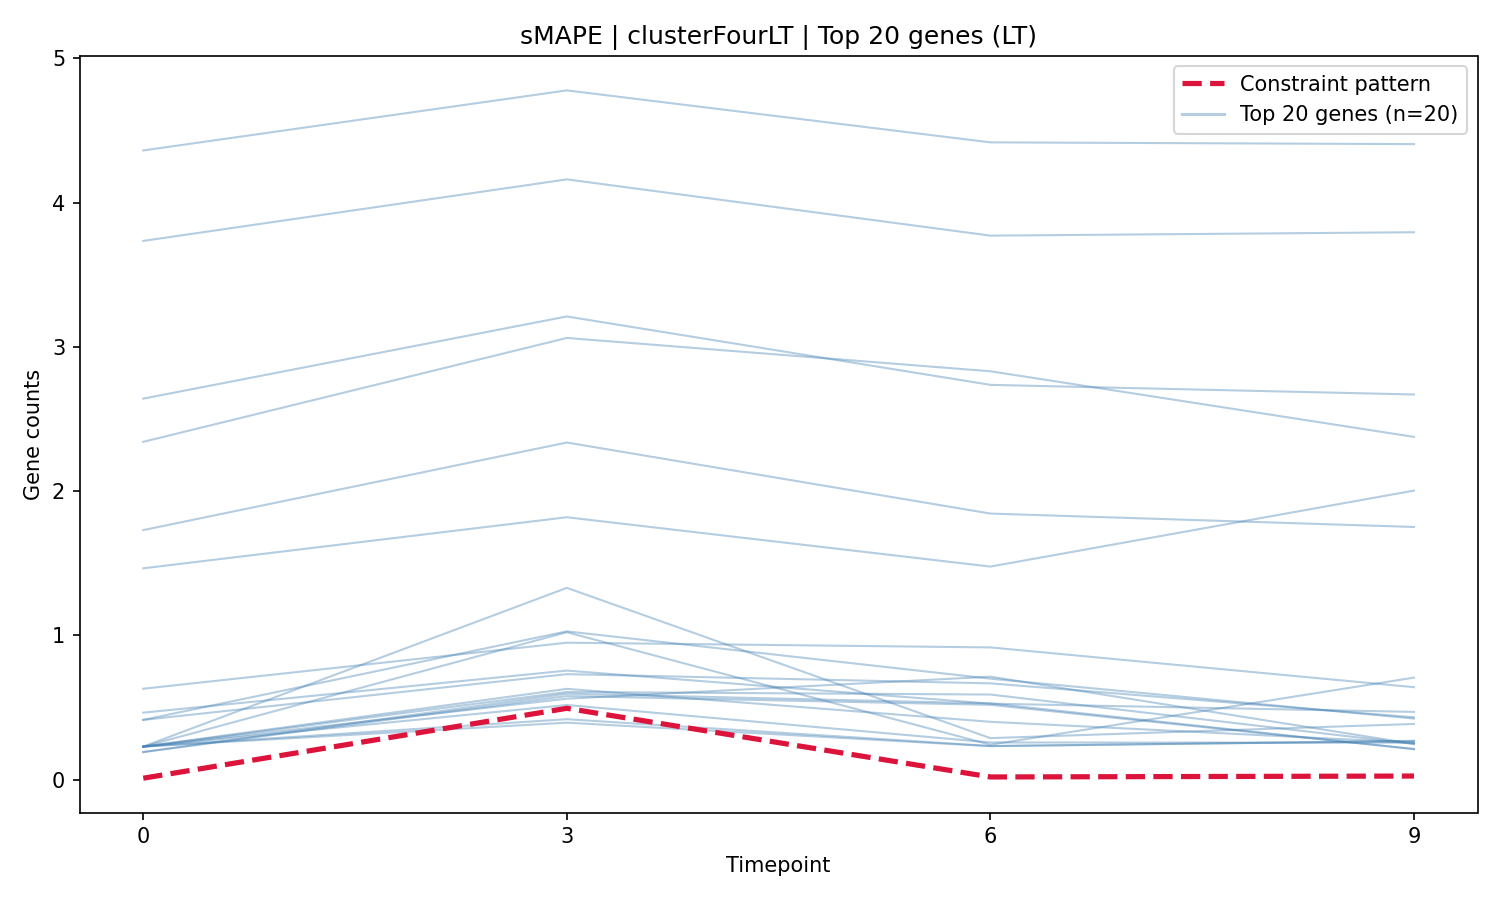
\includegraphics[height=0.85\textheight]{plots/sMAPE_LT_clusterFourLT_constraint.png}
\end{frame}

\begin{frame}{clusterFour LT — Ensemble}
\centering
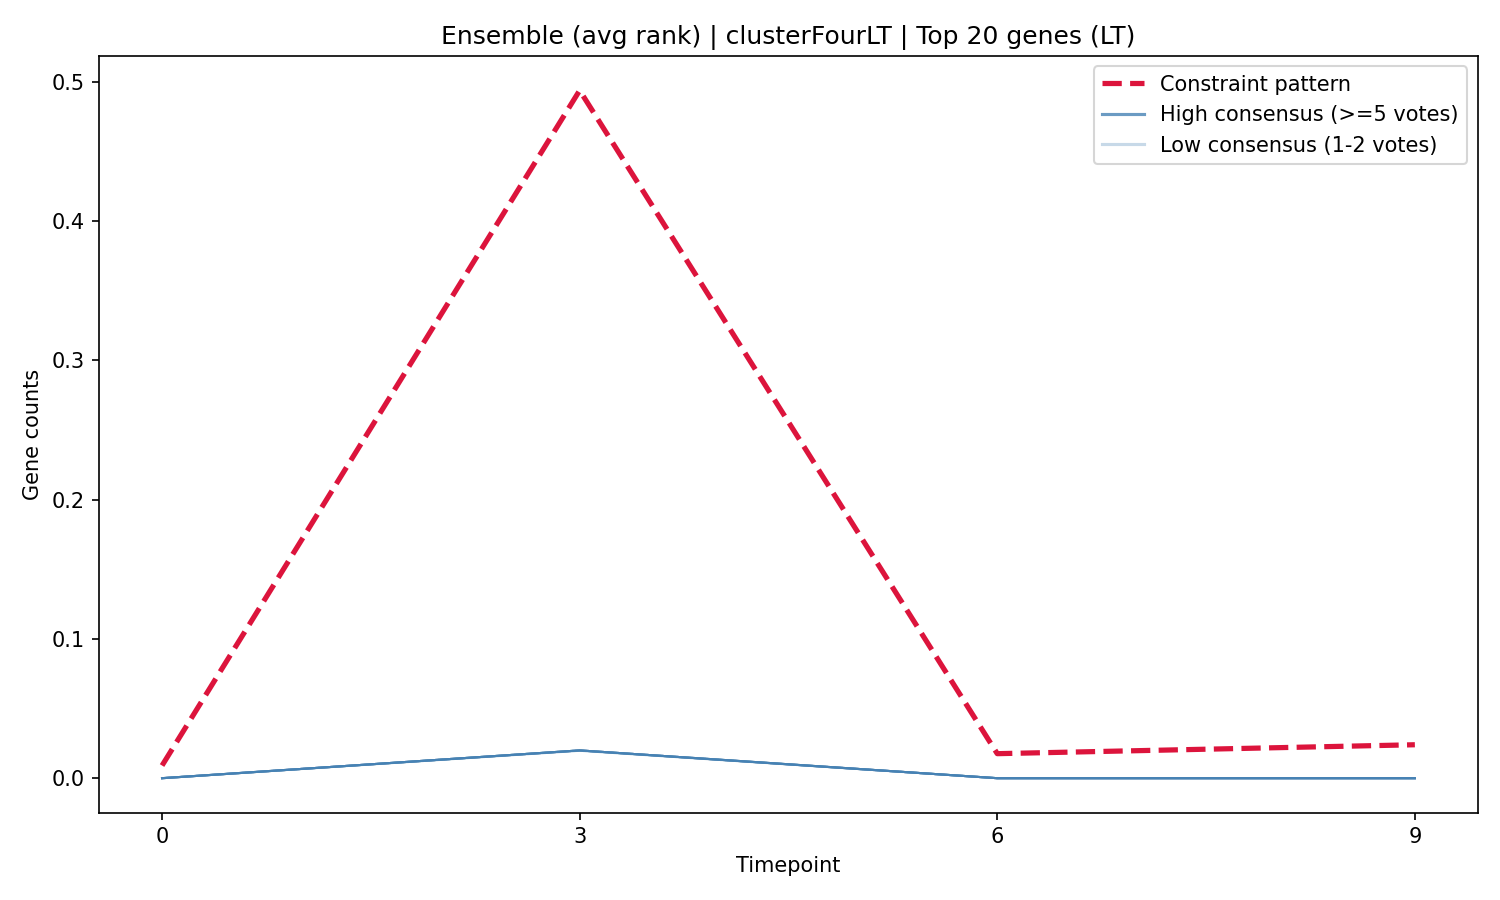
\includegraphics[height=0.85\textheight]{plots/Ensemble_LT_clusterFourLT_constraint.png}
\end{frame}

\begin{frame}{clusterFour LT — Overlap Heatmap}
\centering
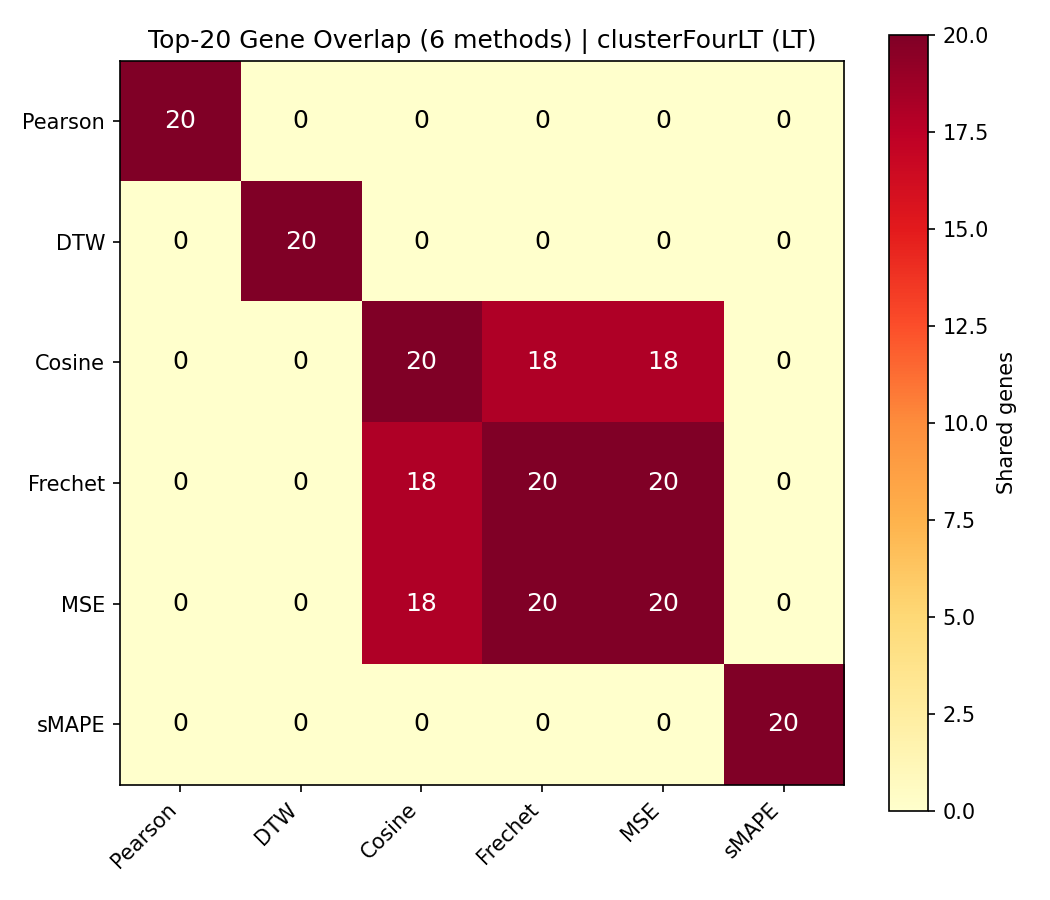
\includegraphics[height=0.85\textheight]{plots/overlap_6methods_LT_clusterFourLT.png}
\end{frame}

\end{document}
